%\documentclass[11pt]{report}
%\usepackage{siunitx}
%\usepackage{graphicx}
%\usepackage{multirow}
%\usepackage[table,xcdraw]{xcolor}
%
%\begin{document}
%\setcounter{chapter}{3}
%\tableofcontents



\newpage
\chapter{Numerical modelling of direct-coupled stimulation}
This chapter contains the results of the numerical modelling approaches applied for direct-coupled (DCoupled) electric field setups. This chapter's contents were collected from the following work:
\begin{itemize}
\item \small \textit{''Direct coupled electrical stimulation towards improved osteogenic differentiation of human mesenchymal stem/stromal cells: a comparative study of different protocols.'', João C. Silva and João Meneses, Fábio F.F. Garrudo, Sofia R. Fernandes, Nuno Alves, Frederico Castelo Ferreira, and Paula Pascoal-Faria, work under review at Nature Scientific Reports.} 
\end{itemize}

This chapter's required cell culture procedures were made in collaboration with the SCERG - Stem Cell Engineering Research Group from iBB/IST - Instituto Superior Técnico, Portugal. Results from this work also gave rise to updated versions of the DCoupled electric field stimulation setup presented here and enhanced stimulation protocols applied to bone marrow-derived mesenchymal stem/stromal cells. This subsequent study will be available at:
\begin{itemize}
\item \small \textit{''Synergy between 3D-extruded electroconductive scaffolds and electrical stimulation in enhancing bone regeneration.'', João C. Silva, Pedro Marcelino, João Meneses, Frederico Barbosa, Carla S. Moura,e Ana C. Marques, Joaquim M. S. Cabral, Paula Pascoal-Faria, Nuno Alves, Jorge Morgado, Frederico C. Ferreira, Fábio F. F. Garrudo, work under submission.}
\end{itemize}  





\newpage
\section{Introduction}
The application of a \ac{DCoupled} constant current stimulation protocol constitutes a simple and straightforward approach shown to promote multiple cellular responses, ranging from cell migration to proliferation and differentiation \cite{Guillot-Ferriols2022-wn, Song2007-qr}. Bioelectric cues function alongside chemical gradients, transcriptional networks, and haptic/tensile cues as part of the morphogenetic field that orchestrates individual cell responses \cite{Tseng2013-yx, Da_Silva2020-su, Guillot-Ferriols2022-wn}. Electrical stimulation cues are considered a valuable tool to guide cells into desirable \ac{TE} outcomes and ultimately unlock the potential of tissue engineering approaches for therapeutic applications \cite{Da_Silva2020-su}.

Electric stimulation has been used clinically for over four decades to promote bone healing, mainly as an adjunct to standard fracture care \cite{Bassett1974-rb}. Several \textit{in vitro} and \textit{in vivo} studies have been conducted by applying DCoupled stimulation to undifferentiated stem cells and differentiated osteoblast cells through the use of different setups, electrode or substrate materials and a variety of waveforms \cite{Guillot-Ferriols2022-wn, Ryan2021-tq, Thrivikraman2018-su}. Accordingly, a study performed by Wang \textit{et al.} demonstrated that a current-base DCoupled protocol (4 \si{\micro\ampere}, 3 \si{\hour} per day for 14 days) enhanced significantly the proliferation and osteogenic differentiation of MC3T3-E1 preosteoblastic cells \cite{Wang2021-tm}. Moreover, Srirussamee and colleagues reported that a daily direct electrical stimulation of 2.2 \si{\volt} for 1 \si{\hour} during a total period of 7 days promoted the \textit{in vitro} osteogenesis of human bone marrow-derived \ac{MSCs}, as evidenced by the significant upregulation of bone-specific marker gene SPP1 \cite{Srirussamee2021-cj}. Mesenchymal stem/stromal cells are a promising cell source for bone repair and have been playing a significant role in \ac{BTE} strategies due to their ability to differentiate towards osteogenic lineage, accumulating other selective advantages like their high availability (since they reside in many organs and tissues of the body), their high in vitro proliferation capacity, low immunogenicity and advantageous immunomodulatory/trophic features \cite{Arthur2020-bs, Silva2020-sw}. Bone marrow-derived MSCs (BMSCs) are considered “gold standard” sources for cell-based therapies, and due to their nature as bone residents, they have been widely used in BTE strategies \cite{Rossi2023-od, Shang2021-ty, Silva2020-dc}. 

The mechanisms behind electrically-driven cellular processes rely on the modulation of membrane potentials by endo or exogenous \ac{EFs} \cite{Thrivikraman2018-su}. The scarcity of predictive models to guide and estimate the experimental \acs{EFs} delivered upon \ac{DCoupled} stimulations has led researchers to rely on the applied input electric potential or on the electric potential drop between the electrodes as a stimulation magnitude comparator between different studies. However, these values do not translate the \acs{EF} effectively delivered to cells, since they do not take into account the critical dielectric properties of the materials involved, the geometry of the electrodes and stimulation chamber, or the complex electrode/electrolyte interface effects \cite{Guette-Marquet2021-rp}. An exception was made by a few studies modelling DC stimulation. Srirussamee \textit{et al.} \cite{Srirussamee2021-cj} designed an electrochemical-based \ac{FEM} model considering a secondary current distribution ruled by Ohm’s law that also accounts for charge transfer reactions, following the Butler-Volmer equation. Two other studies were conducted by Zimmermann \textit{et al.} \cite{Zimmermann2021-fx, Zimmermann2023-gm}. One tackled a \ac{DCoupled} \ac{EF} stimulation \ac{FEM} model that solves Laplace’s equation and accounts for electrode-electrolyte interface interactions, by adjusting the solution to experimental current measurements, and by previously calibrating model parameters with results from electrochemical characterization \cite{Zimmermann2021-fx}. Another work from the same authors presents experimental and numerical methods to calculate the delivered \ac{EF} and current density, including procedures with lumped-element and a \ac{FEM} model approach \cite{Zimmermann2023-gm}. Notably, the widespread implementation of digital models would be highly advantageous to improve current \ac{BTE} methods, since they will allow the optimization of stimulation protocols and the development of predictive platforms, while at the same time reducing experimental time and associated costs \cite{Moller2021-kr, Geris2018-tz}.

The work described in this chapter replicates the \ac{DCoupled} setup originally conceived by Mobini \textit{et al.} \cite{Mobini2016-jh} and further applied in many subsequent studies \cite{Mobini2017-wp, Mobini2017-zr, Leppik2018-bw, Moon2023-rm}. Distinctively from \cite{Mobini2016-jh}, we created a 6-well plate custom lid with L-shaped electrodes made of medical-grade stainless steel wire instead of pure platinum. This work explored the influence of different electric stimulation parameters on \acs{MSCs} osteogenesis. Each applied protocol was guided by an electrical characterization of the \ac{DCoupled} resultant waveform, to individually understand the biological impact of different parts of a typical stimulation waveform. A finite-element model of one of the 6 wells was designed and used to simulate and predict the \ac{EFs} induced by the DCoupled protocols applied. With the results from the developed \ac{DCoupled} setup characterization and correspondent setup digital model, this work also hypothesizes if \ac{DCoupled} electric stimulation performed below the water electrolysis potential remains capable of producing similar osteoinductive effects in \ac{MSCs} as previously reported at higher potentials \cite{Mobini2016-jh, Mobini2017-wp, Mobini2017-zr, Leppik2018-bw}. Also, we explore, with the same constant potential step, what are the differences in terms of osteoinductive effects when applying a very short stimulation exposure versus a more prolonged exposure typical of DCoupled stimulation literature \cite{Mobini2016-jh, Mobini2017-wp, Mobini2017-zr, Leppik2018-bw}. Additionally, the generated protocols allow us to better understand the differences when applying an intermittent step with two distinct frequencies versus a steady electric potential step. A constant current condition was also explored, allowing one of the electrodes to float its potential accordingly. This work contains one of the first studies to directly compare potential-controlled electric stimulation with current-controlled electric stimulation protocols to enhance the osteogenic differentiation of human \acs{MSCs}. All protocols were compared regarding their ability to promote bone marrow-derived \acs{MSCs} viability, proliferation, and osteogenic differentiation.


\section{Aims}
The work described in this chapter has the following main goals:
\begin{itemize}
\item Address the electrode/electrolyte relation in a \acs{BTE} typical \acs{DCoupled} setup;
\item Develop a numerical model to predict the \acs{EF} applied by a custom-developed \acs{DCoupled} setup;
\item Validate the developed model against the reported \acs{EF} from other researchers' \acs{DCoupled} setups;
\item Observe if \acs{DCoupled} electric stimulation, when performed below the water electrolysis potential, remains capable of producing similar osteoinductive effects, as previously reported for \acs{MSCs} subjected to higher potential protocols;
\item Explore differences in \acs{MSCs} effects when subjected to different stimulation protocols parameters: short \acs{DCoupled} stimulation exposure versus a longer exposure; intermittent step waveform with two distinct frequencies; steady electric potential step versus a constant current condition.  
\end{itemize}



\section{Methods}

\subsection{\acs{DCoupled} electrical stimulation system}
Electrical stimulation system custom lids (see Figure \ref{fig4d1}) for a 6-well plate (Falcon\textregistered, Corning, USA) polystyrene tissue culture-treated were designed and \ac{3D} printed in \acs{C8} material (3d4makers, Netherlands) \cite{Meneses2020-dx} by fuse deposition modelling technique (Creatbot F430, Henan Suwei Electronic Technology Co., China). The custom lid computer-aided design files are available for download at Figshare (https://doi.org/10.6084/m9.figshare.23629926.v1). Medical grade stainless steel wire 316LVM (Tegra Medical, Franklin, USA), with a 1 \si{\milli\meter} diameter, was manually bent into an L-shape (width 22 \si{\milli\meter}, height 18 \si{\milli\meter}) and used as electrodes, similarly to Mobini \textit{et al.} \cite{Mobini2016-jh}. Each L-shaped electrode was inserted at its respective hole at the top of the custom lid and glued by a drop of commercial silicone, remaining separated by a distance of 25 \si{\milli\meter} to the next electrode in the same well (Figure \ref{fig4d1} (a)-(c)). The described electrode pair per well constitutes the \ac{DCoupled} electric stimulation system.

Every row of three wells was connected to guarantee that the same electrical current and, correspondingly, the same \acs{EF} were applied across these three wells. Figure \ref{fig4d1}(d) shows the electrical connection schematic. Each row ($n=3$) was then subjected to an electric potential or electric current, with duration and characteristics according to the required stimulation protocol to be applied. The electric potential step application, constant or intermittent, was performed by a lab power source equipment (Tektronix, Berkshire, UK). The electric current application was performed by a custom current source electric circuit (Figure \ref{fig4d2}), composed of an operational amplifier (model TLV 2302), a PNP transistor (model PNP BC 556), and a 100-ohm resistor ($R$), wired according to Figure \ref{fig4d2}. This electric circuit requires a power source ($V_{cc}$) of 12 \si{\volt}, a ground reference, and a potential input ($V_i$) that allows the control and adjustment of the electric current output ($I_e$), following the expression: $I_e=(V_{cc}-V_i)/R$ (see Figure \ref{fig4d2}). The output of each potential or current source condition was measured and validated with a multimeter (ISO-TECH IDM 73, Ahaus, Germany) before its application. 

\begin{figure}
\makebox[\textwidth][c]{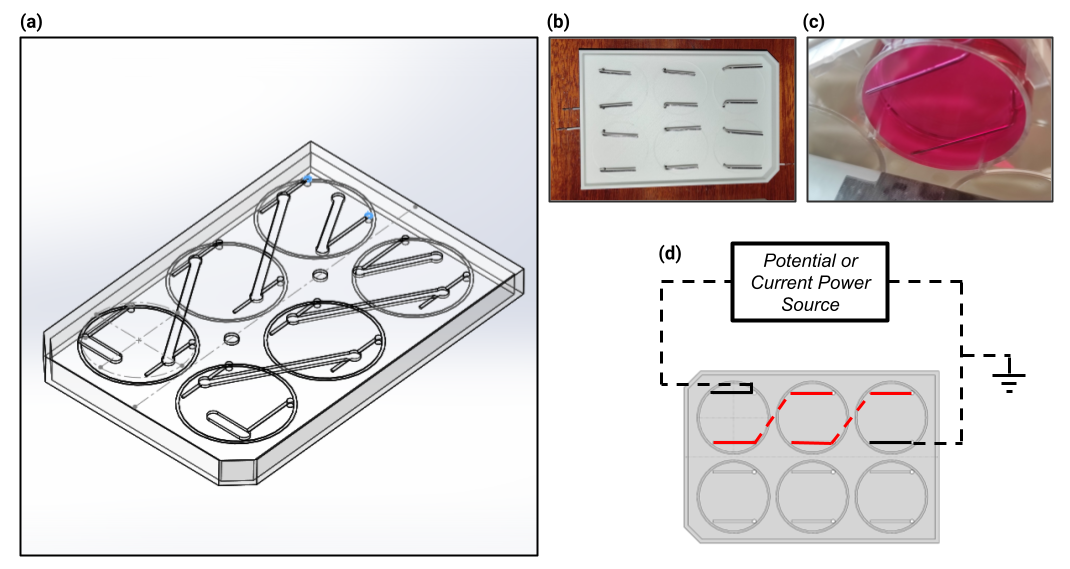
\includegraphics[scale=0.40]{./figures/Figure_4d1.png}}
\caption{\acs{DCoupled} electrical stimulation setup. (a) CAD of the developed custom lid; (b) Bottom view of the custom lid with the L-shape electrodes in medical grade stainless steel wire 316LVM; (c) Bottom view of a single well with electrodes, filled with culture media; (d) Diagram illustrating the electric connection in series of the three wells.}
\label{fig4d1}
\end{figure} 

\begin{figure}
\makebox[\textwidth][c]{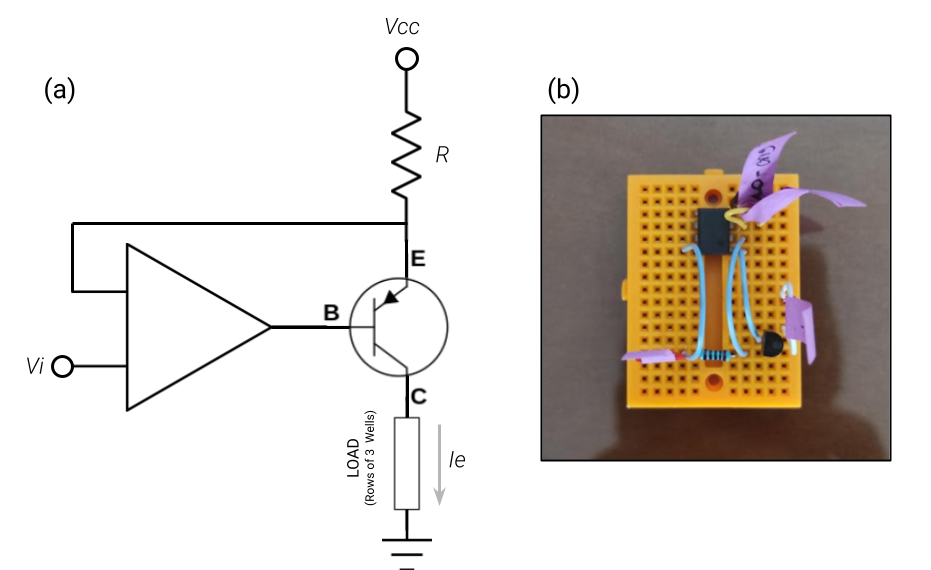
\includegraphics[scale=0.35]{./figures/Figure_4d2.png}}
\caption{Electric circuit of the custom current source developed for the \acs{DCoupled} setup. (a) Diagram of the electric circuit; (b) Image of the corresponding assembled breadboard with the required electronic components.}
\label{fig4d2}
\end{figure} 

\subsection{Determination of culture medium electrical conductivity}
Standard basal media (BM) is composed of Dulbecco’s modified eagle medium (DMEM, Gibco Thermofisher Scientific, Waltham, MA, USA) supplemented with 10\si{\percent} fetal bovine serum (FBS, MSC qualified, Gibco, Thermofisher Scientific) and 1\si{\percent} Antibiotic-antimycotic (Anti-Anti, Gibco, Thermofisher Scientific). Osteogenic culture media (OM) is composed of DMEM + 10\si{\percent} FBS(MSC) + 1\si{\percent} Anti-Anti supplemented with 10 \si{\milli\molar} beta-glycerolphosphate (Sigma-Aldrich, St. Louis, MO-IL, USA), 10  \si{\nano\molar} dexamethasone (Sigma-Aldrich) and 50 \si{\micro\gram\per\milli\liter} ascorbic acid (Sigma-Aldrich). Standard basal culture medium and osteogenic medium electrical conductivities were measured at room temperature (21 - 23 \si{\celsius}) and 37 \si{\celsius} using a multimeter (ISO-TECH IDM 73).
 
\subsection{\acs{DCoupled} electrical stimulation system response characterization}
The response of a single well from the developed \acs{DCoupled} system was studied to determine if the electrode/electrolyte interaction between the stainless steel wire 316LVM and the osteogenic culture medium or basal medium was driven by a faradaic or non-faradaic process. Following the procedure described in the work of Biesheuvel \textit{et al.} \cite{Biesheuvel2018-wu}, we applied an electric current step input to one of the electrodes and fixed the other as ground. The electric potential at the first electrode was probed with an oscilloscope (Keysight DSOX 1102A, Santa Rosa, USA), checking if the resulting curve is likewise the faradaic or non-faradaic typical waveform, as explained by Biesheuvel \textit{et al.} \cite{Biesheuvel2018-wu}. An electric potential step was also applied in the same single well, and the resulting potential waveform at the interface electrode/electrolyte was registered with the same oscilloscope. The response of a row of three wells in series to a potential step of 1.2 \si{\volt} was also acquired to check if the interpretation of a single well result could be expanded to a three-in-a-row configuration. A multimeter (KLEIN TOOLS MM600, Chicago, USA) was used to register the electric current passing these three wells in series to the ground electrode (last well of the row). With this test setup, by applying a range of input potentials (from 0 to 4 \si{\volt}, at increasing steps of 0.5 \si{\volt}), we obtained an I-V curve for the system electrode/electrolyte interactions. The I-V curve was then used to compare the stainless steel wire 316LVM response with previously reported results from different electrode materials. 

\subsection{\acs{EF} predictions from \ac{FEM}}
To predict the \acs{EF} delivered by the \ac{DCoupled} system to the cellular content, a \acs{FEM} analysis was conducted with the AC/DC module of COMSOL Multiphysics (version 5.2a, www.comsol.com, Stockholm, Sweden). The Electric Current (ec) physics interface was selected, considering a stationary study, solving for current conservation (equation \ref{SC1}) and Faraday's law (steady currents derived equation \ref{SC2}).

\begin{equation}
\label{SC1}
\nabla \cdot J = 0
\end{equation}

\begin{equation}
\label{SC2}
\nabla \times E = 0
\end{equation}

\noindent where $J$ is the current density vector and $E$ is the electric field. This equations are then combined to describe materials where the current density is proportional to the electric field, resulting in the constitutional equation known as Ohm's law. Which when solved using the electrostatic potential ($\phi$) and the electric conductivity ($\sigma$) becomes Laplace's fundamental equation for steady currents \ref{SC3}:

\begin{equation}
\label{SC3}
\nabla \cdot (\sigma \nabla \phi) = 0
\end{equation}

A \ac{3D} physics-controlled mesh was generated in COMSOL with the finer mesh option. The model is composed of three material domains, characterized by their electrical conductivity ($\sigma$) and relative permittivity ($\epsilon_r$), according to Figure \ref{fig4d3}: stainless steel 316LVM for electrodes ($\sigma$: \num{1d5} \si{\siemens\per\meter}, $\epsilon_r$: 1); osteogenic culture medium at 37 \si{\celsius} ($\sigma$: \num{1.725} \si{\siemens\per\meter} - determined experimentally as described above, $\epsilon_r$: 80.1 \cite{Visone2018-sa}); polystyrene petri dish ($\sigma$: \num{6.7d-14}  \si{\siemens\per\meter}, $\epsilon_r$: 2.5). An electric potential step of 1.2 \si{\volt} was applied to obtain the current values for the I-V curve (avoiding water electrolysis by staying below the 1.23 \si{\volt} limit \cite{Guette-Marquet2021-rp}). Using this curve, we obtained a peak electric current of 0.17 \si{\milli\ampere}, followed by a drop in current to 0.03 \si{\milli\ampere} (see results section), both measures obtained for the osteogenic medium at 37 \si{\celsius}. These electric current conditions were then added to the model as a floating potential boundary condition to one of the electrodes while setting the other to a ground boundary condition. The average \acs{EF} was calculated at a disk shape region of interest, placed at the center of the well and equidistant from both electrodes (Figure \ref{fig4d3}a, \ref{fig4d3}b, \ref{fig4d3}c). The solution of the model was computed using the conjugate gradients iterative solver.


\begin{figure}
\makebox[\textwidth][c]{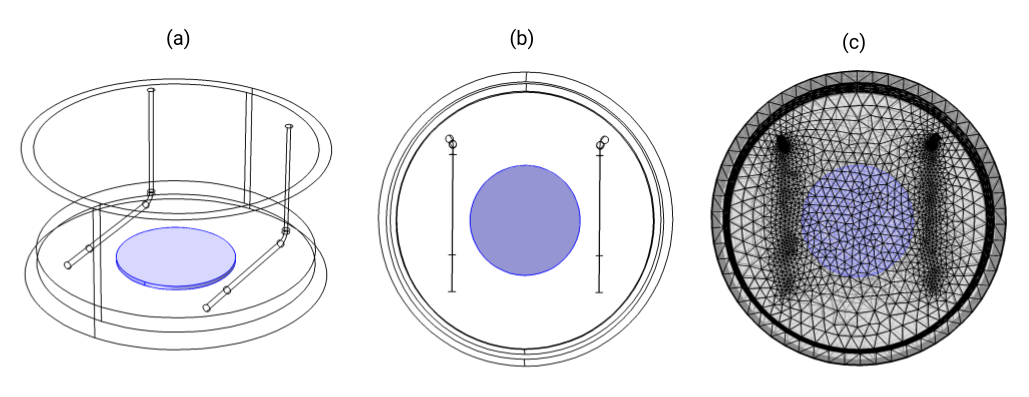
\includegraphics[scale=0.35]{./figures/Figure_4d3.png}}
\caption{\acs{FEM} model geometry of the \acs{DCoupled} setup. The central disk, in blue, represents the ROI under study. (a) Perspective view of the geometry; (b) Top view of the geometry; (c) Top view of the fine mesh.}
\label{fig4d3}
\end{figure}

Due to slight differences between the electrode's sizes, angles, and distances generated when hand-mounted into the custom lid, multiple electrode geometries were modeled inside a single culture well to study and understand the impact of minor geometrical variations on the delivered \acs{EF} prediction. Three geometry variation studies were performed: (1) distances between electrodes, 20 \si{\milli\meter} or 25 \si{\milli\meter}, keeping the same culture medium height and a constant electric current; (2) different culture medium heights, from 2 to 6 \si{\milli\meter}, comparing also between regular or shorter electrodes lengths, $\delta L \pm 5$ \si{\milli\meter}. For this study, we kept the electric current constant at \num{0.05} \si{\milli\ampere}; (3) regular position versus the worst-case tilt scenario, where one of the electrodes has an upper tilt of 5\si{\degree} and the other electrode has a bottom tilt of the same amplitude. Variation study (3) considered the same culture medium height of 5 \si{\milli\meter} and a constant electric current for the two test conditions.

\subsection{FEM model prediction for Mobini \textit{et al.} setup}
The FEM modelling approach described in the previous subsection was also applied to Mobini \textit{et al.} \cite{Mobini2016-jh} setup for \ac{FEM} model validation. Regarding geometric modelling, Mobini \textit{et al.} \cite{Mobini2016-jh} reported a cell culture dish diameter of \num{33.78} \si{\milli\meter} from a 6-well cell culture plate, with 128x85x22 \si{\milli\meter} (produced by TPP, Transadingen, Switzerland). Unfortunately, this well plate device is discontinued for the reported dimensions, but all the remaining models from the same supplier are produced in polystyrene material. The electrode wire has a diameter of 1 \si{\milli\meter} and was made from \num{99.99} \% pure platinum. This wire is reported to have a total length of 50 \si{\milli\meter} bent into an L-shape configuration, with 29-21 \si{\milli\meter} parts. Two electrodes per culture dish were separated by 25 \si{\milli\meter}. It is possible to estimate a wall thickness of 1 \si{\milli\meter} for the entire dish based on recent petri dish models. For the height, it is assumed the reported maximum plate height by the supplier is 22 \si{\milli\meter} (the actual dimension should have been shorter in older models). Also, regarding the reported distance between electrodes and in the absence of a detailed explanation, it was assumed from the wire center axis to the other wire center axis and not from the inner extremities. When trying to consider the inner extremities as the reference, the remaining reported dimensions have been shown to cause a superposition conflict with the reported dish wall position, resulting in an invalid CAD geometry. The distance of the electrodes to the dish bottom is not reported and was assumed to be \num{0.25} \si{\milli\meter}, remaining not in contact with the bottom. The culture medium volume used in each culture dish well was not reported. Still, for similar culture dish dimensions, the Thermo Fisher table about useful numbers in cell culture points \cite{Thermo} recommends a culture medium volume of 2 \si{\milli\liter}. Using this value in the geometrical model, we obtain a liquid volume height of \num{2.26} \si{\milli\meter}. 

Regarding finite element model considerations, the geometric model described in the previous step was imported into COMSOL. Culture dish, electrode and culture medium electrical properties were not measured but otherwise estimated or reported in the Mobini \textit{et al.} \cite{Mobini2016-jh} manuscript. So, to run COMSOL electric currents physics interface, electrical properties for the culture medium were obtained from \cite{Visone2018-sa}, $\sigma$: 1.5 \si{\siemens\per\meter}, $\epsilon_r$: 80.1. For polystyrene material electrical properties were retrieved from \cite{Plastic} with $\sigma$: \num{1.0d-18} \si{\siemens\per\meter} (reported $>$ \num{1.0d18} \si{\ohm\per\meter}), and $\epsilon_r$: 2.6 (interval 2.4 to 3.1). Platinum material $\sigma$ was assumed as \num{9.52d6} \si{\siemens\per\meter} (reported \num{1.05d-9} \si{\ohm\per\meter} \cite{Schuettler2007-zd}), and all metal's relative permittivity for lower frequencies is considered to be 1. The electric stimulus applied in this setup was a 2.2 \si{\volt} DC, as reported in the manuscript, generating an \acs{EF} of 100 \si{\milli\volt\per\milli\meter} (predicted) for this input electrical potential. To translate this to COMSOL, two boundary conditions were applied, one for ground in one electrode tip and another for the measured 0.07 \si{\milli\ampere} current \cite{Srirussamee2019-ai} that translates to a DC floating potential boundary condition on the opposite electrode tip. A normal-sized physics-controlled mesh was created, comprised of 19320 domain elements, 8080 boundary elements, and 721 edge elements. 

\subsection{Electrical stimulation protocol hypothesis}
With the information from the \acs{EF} numerical predictions and the DCoupled system electric response characterization, we created a group of electric stimulation conditions to test some hypotheses (see Figure \ref{fig_t4d1}). Two control cell culture conditions were created with no electrical stimulation protocol, one with basal media and the other with the osteogenic medium. The comparison between them allows us to infer the osteogenic medium effect alone. Then, we tested five cell culture conditions under different DCoupled electric stimulation protocols, all with the osteogenic medium. The potential or current step applied was the same as previously characterized, taking advantage of the characteristic DCoupled system response curve (see results section) when defining the stimulation protocol conditions. All-electric stimulation protocol conditions were applied every two days, stopping when we counted 14 days from the beginning of the experiment.

\begin{figure}
\makebox[\textwidth][c]{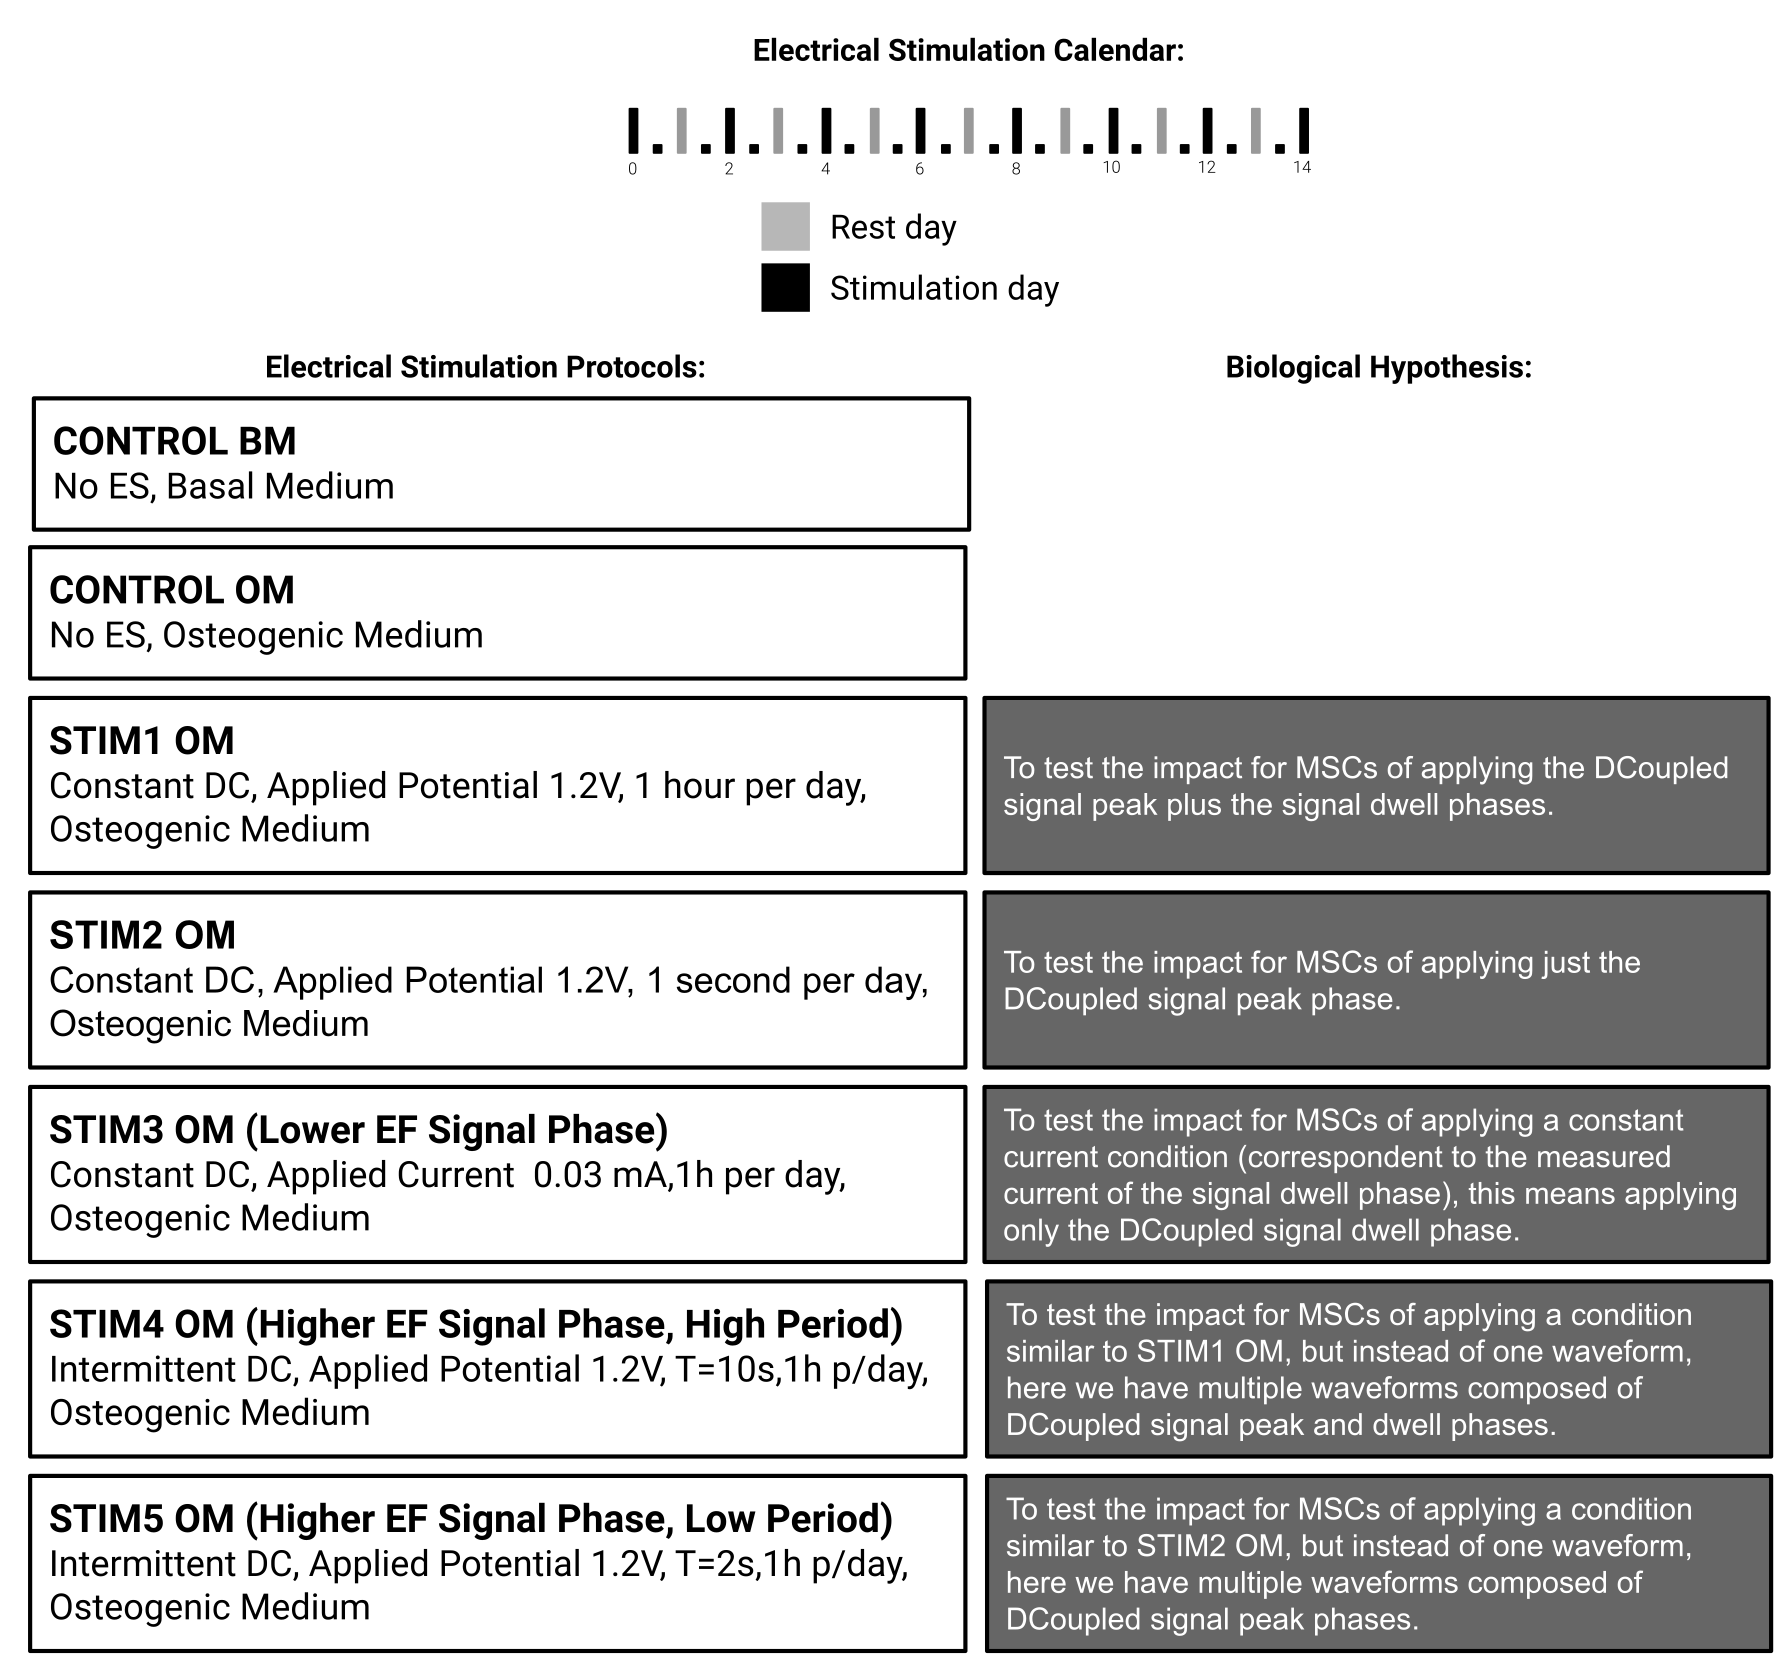
\includegraphics[scale=0.8]{./figures/Table_4d1.png}}
\caption{Infography with DCoupled electrical stimulation protocol description and biological hypothesis under test. Above is the stimulation timeline that was applied to every stimulation condition. Each mentioned protocol reference code will be used in the rest of this chapter to reference a particular protocol.}
\label{fig_t4d1}
\end{figure} 

\subsection{Human \ac{MSCs} culture}
Human bone marrow-derived \ac{MSCs} used in this work were part of the cell bank available at the Stem Cell Engineering Research Group - Institute for Bioengineering and Biosciences (iBB) at Instituto Superior Técnico (IST). Those MSCs were previously isolated according to protocols previously established at iBB-IST \cite{Carvalho2021-ru}. Bone marrow aspirates (Male 46 years) were obtained from Centro Clínico da GNR-Lisboa under previously established collaboration agreements with iBB-IST. An additional sample of fresh, unprocessed bone marrow (Male 24 years) was obtained from Lonza (Switzerland). The human samples were obtained from healthy donors after written informed consent according to Directive 2004/23/EC of the European Parliament and of the Council of March 31, 2004, on setting standards of quality and safety for the donation, procurement, testing, processing, preservation, storage, and distribution of human tissues and cells (Portuguese Law 22/2007, June 29), with the approval of the Ethics Committee of the respective clinical institution. Isolated cells were frozen in liquid/vapor nitrogen tanks until further use. Before the cell culture assays, the \ac{MSCs} were thawed and expanded on tissue culture flasks (T-75 \si{\square\centi\meter}) using low-glucose \acs{DMEM} (Gibco, Thermo Fisher Scientific) supplemented with 10\si{\percent} \acs{FBS} (Gibco, Thermo Fisher Scientific) and 1\si{\percent} Anti-Anti Solution (Gibco, Thermo Fisher Scientific). Cells were kept in an incubator at 37 \si{\celsius} and 5\si{\percent} CO\textsubscript{2} in a humidified atmosphere, and the medium was exchanged every three days. All the experiments were conducted using cells between passages 3 and 5. 

\subsection{Evaluation of the effects of different electric stimulation protocols on MSC proliferation and osteogenic differentiation} 
Human bone marrow-derived \ac{MSCs} were harvested and seeded in 6-well culture plates at a density of 10.000 cells/ \si{\square\centi\meter}. The cells were then cultured for 14 days in an incubator at 37 \si{\celsius} and 5\si{\percent} CO\textsubscript{2} under the different electrical stimulation protocols and respective controls as previously specified in subsection 4.3.6. Culture media (volume of 3 mL per well) were fully renewed every three days. Cell morphology and metabolic activity were monitored throughout the culture after 14 days of culture and exposure to the different electric stimulation protocols, and the osteogenic differentiation of \ac{MSCs} was assessed. 

\subsection{Cell viability and morphology assessment} 
After 14 days of human bone marrow-derived \ac{MSCs} osteogenic differentiation under the different electric stimulation protocols, cell viability was assessed through LIVE/DEAD staining. Briefly, cells were first washed with \ac{PBS}, after which they were incubated in the dark with ethidium bromide (2 \si{\micro\molar}) (Sigma-Aldrich) and calcein (4 \si{\micro\molar}) (Sigma-Aldrich) solution (prepared in \ac{PBS}) for 1 hour. Fluorescence images were obtained using a LEICA DMI3000B inverted fluorescence microscope (Leica Microsystems). 

Cell morphology was observed and imaged at several culture time points using bright-field microscopy (LEICA DMI3000B, Leica Microsystems). At the end of the protocol (day 14), the morphology of the cells was also observed after staining with 4,6-diamidino-2-phenylindole dihydrochloride (DAPI, nuclei stains in blue) and Phalloidin (actin cytoskeleton stains in red). For that, the cultures were firstly washed with \ac{PBS}, fixed in 4\si{\percent} paraformaldehyde (Sigma-Aldrich) solution (in \ac{PBS}) for 20 minutes and permeabilized in a 0.1\si{\percent} Triton X-100 solution (Sigma-Aldrich) in \ac{PBS} for 10 minutes. Afterward, cells were incubated with Phalloidin-TRITC (2 \si{\micro\gram\per\milli\liter} in PBS; Sigma Aldrich) and protected from light for 45 minutes. Samples were then washed with \ac{PBS} and counterstained with DAPI (1.5 \si{\micro\gram\per\milli\liter} in \ac{PBS}; Sigma-Aldrich) for 5 minutes. Finally, the cultures were rewashed with PBS, and the fluorescence staining was imaged using an inverted fluorescence microscope (LEICA DMI3000B, Leica Microsystems). 

\subsection{Metabolic activity assay} 
The metabolic activity of differentiating human bone marrow-derived \ac{MSCs} under the different electric stimulation protocols (and respective controls) was evaluated on days 3, 7, and 14 using the AlamarBlue assay (AlamarBlue Cell Viability Reagent; Thermo Fisher Scientific) following the manufacturer’s guidelines. Briefly, a 10\si{\percent} (v/v) AlamarBlue solution diluted in cell culture media was added to the cell cultures and incubated at 37 \si{\celsius} and 5\si{\percent} CO\textsubscript{2} in a humidified atmosphere for 3 \si{\hour}. Fluorescence intensity was measured in a microplate reader (Infinite 200 Pro; TECAN) at an excitation/emission wavelength of 560/590 \si{\nano\meter}. For each experimental group, the fluorescence intensity was analyzed in 3 independent samples ($n=3$), and the fluorescence values of each sample were measured in triplicates. 

\subsection{Alkaline phosphatase activity assay} 
\acs{ALP} activity, which is associated with bone formation and osteoblast function \cite{Nakamura2020-zx}, was quantified using a colorimetric \ac{ALP} quantification kit (BioAssays Systems) following the manufacturer’s guidelines. \ac{ALP} activity was assessed after 14 days of osteogenic differentiation under the different electric stimulation protocols. Cultures were firstly washed with \ac{PBS}, and lysates were obtained after incubation in a 0.2\si{\percent} Triton X-100 (Sigma-Aldrich) solution (prepared in \ac{PBS}) overnight at room temperature and under agitation. Afterward, a p-nitrophenyl solution (10 \si{\milli\molar}) was added to the lysates. The absorbance was measured on a microplate reader (Infinite 200 Pro; TECAN) at 405 \si{\nano\meter}. For each experimental group, the absorbance was quantified for three independent samples ($n=3$), and values for each sample were measured in triplicates. \ac{ALP} activity values were calculated following the manufacturer’s protocol and normalized to the cell metabolic activity of each sample.  

\subsection{Calcium quantification assay} 
The calcium content levels produced by human bone marrow-derived \ac{MSCs} under osteogenic differentiation and submitted to the different electric stimulation protocols for 14 days were determined using a calcium colorimetric assay kit (Sigma-Aldrich). First, cells were washed with \ac{PBS} and incubated in a 1\si{\molar} HCl solution overnight (with agitation). Afterward, the supernatant was collected and used for calcium determination, following the manufacturer’s instructions. Briefly, three independent samples of each experimental condition ($n=3$) and diluted forms of a Calcium Standard Solution (500 \si{\milli\molar}) available in the kit were pipetted into a 96-well plate at several concentrations. Afterward, a Chromogenic Reagent and a Calcium Assay buffer (provided in the kit) were added to each well, and the solutions were gently mixed. The samples were incubated for 10 min in the dark at room temperature. The absorbance was measured on a microplate reader (Infinite 200 Pro; TECAN) at 575 \si{\nano\meter} (duplicate measurements per sample). The absorbance measurements for the different Calcium Standard Solution concentrations were used to develop a calibration curve, which was used to estimate the concentration of calcium present in each sample. The values were normalized to the cell metabolic activity of the respective sample.

\subsection{Osteogenic stainings} 
\ac{ALP}/Von Kossa, Alizarin Red, and Xylenol Orange stainings are often used to confirm the osteogenic differentiation of \ac{MSCs} through the detection of the bone \ac{ECM} markers (\ac{ALP} and mineral deposits) \cite{Zhou2021-av}. In this study, the stainings were performed after 14 days of osteogenic differentiation under the different electric stimulation protocols. After being washed with \ac{PBS} and fixed with 4\si{\percent} paraformaldehyde for 20 min, the human bone marrow-derived \ac{MSCs} were first washed twice with milliQ and stained for ALP presence by incubation in a solution comprised of 0.1 \si{\molar} TRIS-HCl (Sigma-Aldrich), containing Fast Violet Solution (Sigma-Aldrich) and Naphthol AS MX-P04 (Sigma-Aldrich) for 45 min. The cells were then washed three times with \ac{PBS} and kept in milliQ water while being observed under the microscope (LEICA DMI3000B, Leica Microsystems). After washing the samples with \ac{PBS}, Von Kossa staining was performed on the same samples by incubating them in a 2.5\si{\percent} silver nitrate solution (Sigma-Aldrich) for 30 min. Finally, the cultures were washed three times with \ac{PBS}, once with miliQ water, and kept in milliQ water until observation under the microscope (LEICA DMI3000B). 

Alizarin red staining of the cells from different experimental groups was performed to detect the calcium deposits. Paraformaldehyde-fixed samples were incubated in a 2\si{\percent} Alizarin red (Sigma-Aldrich) solution (in \ac{PBS}) for 1 hour at room temperature. The cultures were washed afterward multiple times with \ac{PBS} and milliQ water, after which they were imaged with an inverted fluorescence microscope (LEICA DMI3000B).  

To further confirm the presence of mineral deposits within the samples after 14 days of human bone marrow-derived \ac{MSCs} osteogenic differentiation under the different electric stimulation protocols, a 20 \si{\milli\molar} Xylenol Orange solution (Sigma-Aldrich) was added to previously fixed samples for 1 hour at room temperature. Cells were then washed successively with \ac{PBS}, and the fluorescence staining was imaged using an inverted fluorescence microscope (LEICA DMI3000B).

\subsection{\acs{RNA} isolation, conversion to complementary \acs{DNA}, and quantitative real-time polymerase chain reaction (\acs{RT-qPCR}) analysis} 

After the osteogenic differentiation of human bone marrow-derived \ac{MSCs} under the different electric stimulation protocols for 14 days, cells were harvested from the plates, centrifuged, and the obtained pellets were stored at -80 \si{\celsius} until further use. \ac{RNA} extraction from cell pellets was performed using the RNeasy Mini Kit (QIAGEN) according to the manufacturer’s guidelines. Afterwards, the \ac{RNA} concentration of the different samples was quantified using a NanoVue Plus spectrophotometer (GE Healthcare).  

Complementary \ac{DNA} was synthesized from the purified \ac{RNA} using the High-Capacity complementary \ac{DNA} Reverse Transcription Kit (Applied Biosystems) according to the manufacturer’s protocol. Reaction mixtures comprised of 10 \si{\micro\liter} of MasterMix – constituted by 2 \si{\micro\liter} of RT 10x buffer, 0.8 \si{\micro\liter} of dNTP mix, 4.2 \si{\micro\liter} of RNase-free water, 2 \si{\micro\liter} of random primers and 1 \si{\micro\liter} of Multiscribe Reverse Transcriptase – and 10 \si{\micro\liter} of purified \ac{RNA} sample were mixed and placed in a T100TM thermal cycler (Bio-Rad) for 5 minutes at 25 \si{\celsius}, 20 minutes at 46 \si{\celsius} and 1 minute at 95 \si{\celsius}, and then were maintained at 4 \si{\celsius}.  

\acs{RT-qPCR} analysis was performed using a StepOnePlus real-time polymerase chain reaction system (Applied Biosystems) and NZYSpeedy qPCR Green Master Mix (2x), ROX plus (Nzytech) following the manufacturer’s protocol. The reactions were carried out at 95 \si{\celsius} for 10 minutes, followed by 40 cycles of 95 \si{\celsius} for 15 seconds and 60 \si{\celsius} for 1 minute. All samples were analyzed in triplicates ($n=3$). The results obtained were analyzed using the 2-\si{\Delta\Delta}Ct method to determine relative changes in specific target genes (ALP, RUNX2, COL1A1, OPN, OC, CACNA1C, and SCN1\si{\alpha}) expression compared with the control sample (human bone marrow-derived \ac{MSCs} at day 0 before seeding). Gene expression was primarily normalized to the housekeeping gene glyceraldehyde-3-phosphate (GADPH) expression and then calculated as a fold-change relative to the baseline expression of the target genes in the control sample. The primer sequences used in the \ac{RT-qPCR} analysis are presented in Table \ref{tabPrimers}.

\begin{table}
\caption{Primer sequences used in the RT-qPCR analysis.}
\bigskip
\scriptsize
\centering
\begin{tabularx}{350px}{lll} \toprule[0.25em]
\multicolumn{1}{l}{\textbf{GENE}} & \textbf{FWD PRIMER SEQUENCE} & \textbf{REV PRIMER SEQUENCE} \\ \cmidrule(r){1-3}
GAPDH & \textit{5’-GGTCACCAGGGCTGCTTTTA-3’} & \textit{5’-CCTGGAAGATGGTGATGGGA -3’} \\
ALP & \textit{5’- ACCATTCCCACGTCTTCACATTT-3’} & \textit{5’- AGACATTCTCTCGTTCACCGCC-3’} \\
Runx2 & \textit{5’-AGATGATGACACTGCCACCTCTG-3’} & \textit{5’-GGGATGAAATGCTTGGGAACT-3’} \\
COL1A1 & \textit{5’-CATCTCCCCTTCGTTTTTGA-3’} & \textit{5’-CCAAATCCGATGTTTCTGCT-3’} \\
OPN & \textit{5’-CAGGTCTGCGAAACTTCTTAG-3’} & \textit{5’-CTCCATTGACTCGAACGACTC-3’} \\
OC & \textit{5’-TGTGAGCTCAATCCGGCATGT-3’} & \textit{5’-CCGATAGGCCTCCTGAAGC-3’} \\
CACNA1C & \textit{5’-GTACAAAGACGGGGAGGTTGAC-3’} & \textit{5’-GTAGTTGTAGATGGGGCCCTTG-3’} \\
SCN1\si{\alpha} & \textit{5’- TTGTGACGCTTAGCCTGGTAG-3’} & \textit{5’- ACGATGATGGCCAAGACGAG-3’} \\ \bottomrule[0.25em] 
\end{tabularx}
\label{tabPrimers}
\end{table} 

\subsection{Immunofluorescence analysis of bone-specific proteins} 
Immunofluorescence analysis evaluated the presence of type I collagen, osteopontin, and osteocalcin (relevant proteins produced during bone \acs{ECM} formation) within the cultures after 14 days of osteogenic differentiation under the different electric stimulation protocols. Previously fixed (paraformaldehyde 4\si{\percent} for 20 minutes) samples were washed twice in \acs{PBS}, after which the scaffolds were immersed in a permeabilization/blocking solution comprised of 1\si{\percent} \ac{BSA} (Sigma-Aldrich), 10\si{\percent} \acs{FBS} and 0.03\si{\percent} Triton X-100 for 45 min at room temperature. Solutions containing primary antibodies for type I collagen (MA1-26771, Thermo-Fischer), osteopontin (ab8448, Abcam) and osteocalcin (MAB1419, R\&D Systems) (1:200 in 1\si{\percent} \acs{BSA}, 10\si{\percent} \acs{FBS}, 0.03\si{\percent} Triton X-100 solution) were then incubated with the respective samples overnight at 4 \si{\celsius}. Cells were then incubated with the secondary antibodies (1:200 in 1\si{\percent} \acs{BSA}; goat anti-mouse IgG-AlexaFluor 546 (Thermo Fisher Scientific) for type I collagen and goat anti-rabbit IgG-AlexaFluor 546 (Thermo Fisher Scientific) for osteopontin and osteocalcin) for 1 hour at room temperature in the dark. Following two washes with \ac{PBS}, the samples were counterstained with DAPI (1.5 \si{\micro\gram\per\milli\liter} in \ac{PBS}) for 5 min at room temperature, washed twice with \ac{PBS} and imaged using a fluorescence microscope (LEICA DMI3000B). 

\subsection{Statistical analysis}
When applicable, results are presented as average values $\pm$ standard deviation (SD). All the in vitro cell culture experiments were performed using three independent samples ($n=3$) from two different donors unless specified otherwise. Statistical analysis of the data was performed by one-way ANOVA, followed by a Tukey post-hoc test using the GraphPad Prism 7.0 software (GraphPad, San Diego, CA, USA). Data were considered statistically significant when the p-values obtained were less than 0.05 (95\si{\percent} confidence intervals, $*p<0.05$). 




\section{Results}


\subsection{Electrode/electrolyte interface characterization}
The response of a DCoupled system single well (filled with osteogenic culture medium) to an electric current square wave input followed the predicted response for a faradaic process. Such behavior differs from a typical non-faradaic process, as shown in Figure \ref{fig4d4}a,b. Moreover, replacing the osteogenic culture medium with basal medium resulted in the same response curve shape, meaning that a faradaic process also drives basal medium interaction with stainless steel wire 316LVM. We further confirmed the electrode/electrolyte interface faradaic process by analyzing the response to an electric potential step, since the response curve shape followed exactly the waveform indicated by Biesheuvel \textit{et al.} \cite{Biesheuvel2018-wu} (Figure \ref{fig4d4}c). This potential step response curve is characterized by an initial signal peak (higher potential and current) when the input potential step is applied, followed by a decrease in the electric potential until it reaches a stable signal dwell (lower potential and current). The developed system, composed of a series of three wells, showed the same response (Figure \ref{fig4d5}a), attenuated by the fact that the overall electric resistance of the system is at least three times higher than the electric resistance of a single well. The I-V curve for these three wells in a series setup is also shown in Figure \ref{fig4d5}b. We digitized the curve obtained by Srirussamee \textit{et al.} \cite{Srirussamee2021-cj} (red line in Figure \ref{fig4d5}b) and observed that our stable curve and theirs are similar in shape. The divergence observed in the values may be attributed to the different electrode/electrolyte species involved. We clarify that the stable curve in Figure \ref{fig4d5}b represents the value of the electric current in the signal dwell phase. In contrast, the peak curve represents the maximum current achieved when the input signal is applied to the three wells in the series setup. The applied potential of 1.2 \si{\volt} was chosen deliberately below the water electrolysis limit of 1.23 \si{\volt} \cite{Guette-Marquet2021-rp} to test if DCoupled electric stimulation performed below the water electrolysis potential remains capable of producing similar osteoinductive effects as previously reported at higher potentials \cite{Mobini2017-wp, Mobini2017-zr, Leppik2018-bw}. When 1.2 \si{\volt} is applied to our setup, we measured a peak electric current of 0.17 \si{\milli\ampere} (during signal peak) preceding a current drop to 0.02 - 0.03 \si{\milli\ampere} (during signal dwell). Dwell current showed to be slowly dropping with time. Regarding the electric current controlled hypothesis, a constant current condition of 0.03 \si{\milli\ampere} generated electrode potential differences that grew above the water electrolysis limit, registering a maximum potential difference of 3.74 \si{\volt} for one electrode pair in a three-well series. The results from this characterization process allowed us to create the protocol conditions described in the methods section, disaggregating the part of the waveform responsible for the higher current and higher \acs{EF} from the part responsible for the lower current and lower \acs{EF}.    

\begin{sidewaysfigure}
\makebox[\textwidth][c]{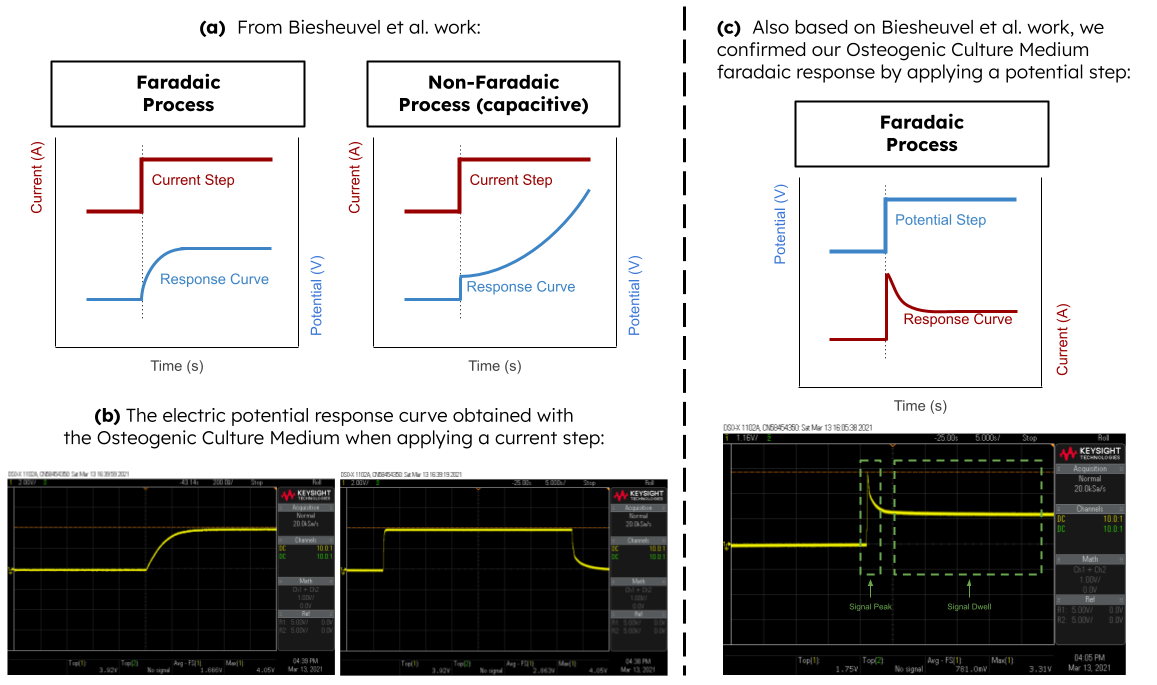
\includegraphics[scale=0.50]{./figures/Figure_4d4.png}}
\caption{Responce characterization of a DCoupled system accordingly to Biesheuvel \textit{et al.} \cite{Biesheuvel2018-wu}: (a) Reference Faradaic versus Non-Faradaic expected responses for an applied current step; (b) Oscilloscope print screens for the measured responses of the custom developed DCoupled system for a current step input, showing a Faradaic process response. At the vertical axis is presented the electric potential and at the horizontal axis is the time; (c) Reference versus oscilloscope print screen for the measured responses of the custom-developed DCoupled system for a potential step input. In the potential step response (c), the peak and dwell phases of the waveform are identified.}
\label{fig4d4}
\end{sidewaysfigure}

\begin{sidewaysfigure}
\makebox[\textwidth][c]{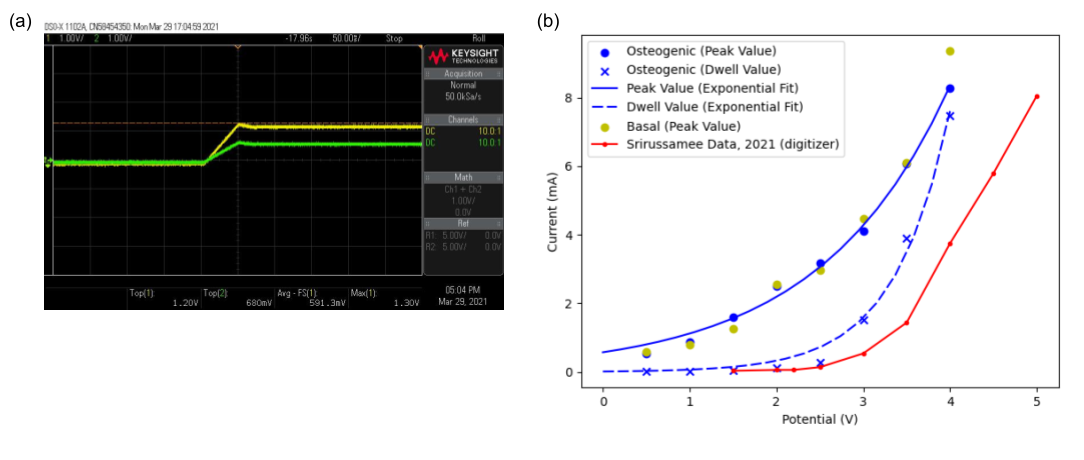
\includegraphics[scale=0.50]{./figures/Figure_4d5.png}}
\caption{Response of the developed DCoupled setup with three wells in series: (a) Oscilloscope print screen for the potential step input response. It shows the measurements at the first (yellow curve) and last electrode (green curve) in the three wells array; (b) Comparison between the obtained I-V curve (maximum and stable forms, in blue) and curve data from Srirussamee \textit{et al.} \cite{Srirussamee2021-cj} (in red; obtained with a digitizer).}
\label{fig4d5}
\end{sidewaysfigure}


\subsection{Computational modelling of the \acs{EF}}
Before the \acs{FEM} analysis of the \acs{EF}s generated within the electric stimulation setup, the electrical conductivities of both basal (BM) and osteogenic (OM) culture media were determined. For typical room temperatures of 21 - 23 \si{\celsius}, the electrical conductivity values were 1.383 \si{\siemens\per\meter} (OM) and 1.392 \si{\siemens\per\meter} (BM). Increasing the media temperature to 37 \si{\celsius} also increased its electrical conductivity to 1.741 \si{\siemens\per\meter} (OM) and 1.725 \si{\siemens\per\meter} (BM). The values measured follow the ones reported by Mazzoleni \textit{et al} \cite{Mazzoleni1986-wp}. 

\ac{FEM} solutions were obtained using the conjugate gradients iterative solver, that quickly converged (less than 10s). Mesh independence was confirmed by repeating the calculation of the obtained results with the COMSOL extremely fine element size option. Slight geometrical deviations were introduced into the developed model to study the impact of such differences in the \acs{EF} magnitude. Changing the distance between electrodes from 20  to 25 \si{\milli\meter} (while keeping the culture medium volume height constant and a constant electric current input) showed no difference in the \acs{EF} predictions larger than 0.01 \si{\volt\per\meter}, stating that minor geometric deviations do not impact on this particular setup. The impact of culture media height changes was also studied (ranging from 2 \si{\milli\meter} to 6 \si{\milli\meter} in steps of 1 \si{\milli\meter}) at the same constant electric current magnitude and distance between the electrodes. The predicted \acs{EF} changes by almost 30\si{\percent} per milliliter of culture medium added or removed. This result indicates that each well should have the same volume of culture medium. In this study, we used 3 \si{\milli\liter} of culture medium per well of a standard 6-well culture plate, corresponding to a height of approximately 3.5 \si{\milli\meter}. At a constant electric current and culture medium height, changing the electrode length to more or less 5 \si{\milli\meter} will have a maximum impact of 6\si{\percent} in the predicted \acs{EF}. Also, under the same conditions, twisting 5\si{\degree} up/down one or both electrodes corresponds to a maximum variation of 0.09\si{\percent} in the predicted \acs{EF}, representing only a residual impact in this setup (Tables \ref{tab4d1},\ref{tab4d2},\ref{tab4d3}). Our modelling method applied to Mobini \textit{et al.} \cite{Mobini2016-jh} setup predicts an average \acs{EF} in the cell culture medium of 0.59 \si{\volt\per\meter}. The solution converged in 2 seconds, and as previously stated in the methods section, it considered the resulting current of 0.07 \si{\milli\ampere} as reported by Srirussamee \textit{et al.} \cite{Srirussamee2019-ai} and geometry approximations as reported in the original Mobini \textit{et al.} manuscript. 

Numerical \ac{FEM} models of the developed setup predicted an average culture medium \acs{EF} in each of the three wells of 1.48 \si{\volt\per\meter} during the signal peak phase and 0.26 \si{\volt\per\meter} during the signal dwell phase (Figure \ref{fig4d6}a, \ref{fig4d6}b).


\begin{figure}
\makebox[\textwidth][c]{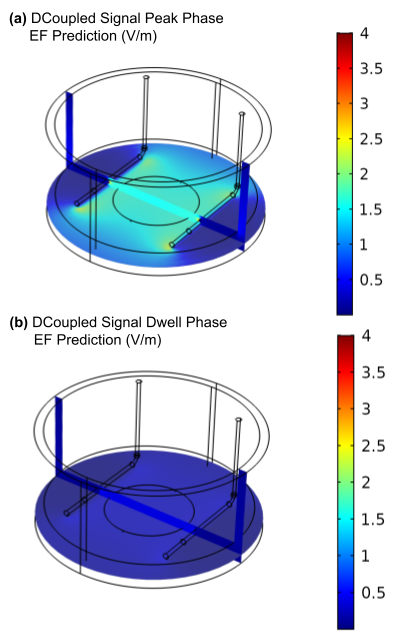
\includegraphics[scale=0.65]{./figures/Figure_4d6.png}}
\caption{FEM numerical model of the developed DCoupled setup: (a) EF prediction for the signal peak electric current of 0.17 \si{\milli\ampere}; (b) EF prediction for the signal dwell electric current of 0.03 \si{\milli\ampere}.}
\label{fig4d6}
\end{figure}

\begin{table}
\caption{Predicted impact of electrodes distance in the DCoupled setup \acs{EF} stimulation delivery at the \acs{ROI}, considering 2 \si{\milli\meter} of culture medium height, 20/25 \si{\milli\meter} distance.}
\bigskip
\small
\centering
\begin{tabularx}{280px}{lll} \toprule[0.15em]
 \textbf{Distance Between Electrodes} & \multicolumn{2}{l}{\textbf{Electric Field}} \\ \cmidrule(l){2-3}
 & 0.03 \si{\milli\ampere} & 0.17 \si{\milli\ampere} \\ \cmidrule(r){1-3}
25 \si{\milli\meter}  & 0.33 \si{\volt\per\meter} & 1.88 \si{\volt\per\meter} \\
20 \si{\milli\meter}  & 0.33 \si{\volt\per\meter} & 1.88 \si{\volt\per\meter} \\ \bottomrule[0.15em] 
\end{tabularx}
\label{tab4d1}
\end{table}


\begin{table}
\caption{Well liquid volume variation impact in the DCoupled setup \acs{EF} stimulation delivery at the \acs{ROI}, for a constant electric current of 0.05 \si{\milli\ampere}. The green values indicate the variation in the \acs{EF} due to liquid volume change. In contrast, the red values indicate the variation imposed by the longer versus shorter electrodes ($\pm$ 5 \si{\milli\meter} size).}
\bigskip
\small
\centering
\begin{tabularx}{\textwidth}{lll} \toprule[0.25em]
 \textbf{Liquid Height} &  \textbf{Electric Field, Long Electrodes} &  \textbf{Electric Field, Short Electrodes} \\ \cmidrule(r){1-3}
2 \si{\milli\meter} & 0.55 \si{\volt\per\meter} & 0.58 V/m (\textcolor{red}{+5\%}) \\ 
3 \si{\milli\meter} & 0.37 \si{\volt\per\meter} (\textcolor{green}{-32\%}) & 0.38 V/m (\textcolor{red}{+3\%}) \\ 
4 \si{\milli\meter} & 0.27 \si{\volt\per\meter} (\textcolor{green}{-27\%}) & 0.28 \si{\volt\per\meter} (\textcolor{red}{+4\%}) \\ 
5 \si{\milli\meter} & 0.22 \si{\volt\per\meter} (\textcolor{green}{-18\%}) & 0.23 \si{\volt\per\meter} (\textcolor{red}{+5\%}) \\ 
6 \si{\milli\meter} & 0.18 \si{\volt\per\meter} (\textcolor{green}{-18\%}) & 0.19 \si{\volt\per\meter} (\textcolor{red}{+6\%}) \\ \bottomrule[0.25em] 
\end{tabularx}
\label{tab4d2}
\end{table}


\begin{table}
\caption{Worst case scenario impact in the DCoupled setup \acs{EF} stimulation delivery at the \acs{ROI}, considering a twist angle 5º up/down and a constant 5 \si{\milli\meter} culture medium height. The variation value, presented by the red color, was calculated by comparison with the no-twist scenario under the same conditions.}
\bigskip
\small
\centering
\begin{tabularx}{200px}{ll} \toprule[0.15em]
\textbf{Electric Current} &  \textbf{Electric Field}  \\ \cmidrule(r){1-2}
0.03 \si{\milli\ampere} & 0.133 \si{\volt\per\meter} (\textcolor{red}{0.09\%}) \\ 
0.17 \si{\milli\ampere} & 0.75 \si{\volt\per\meter} (\textcolor{red}{0.09\%})  \\ \bottomrule[0.15em] 
\end{tabularx}
\label{tab4d3}
\end{table}



\subsection{Effects of electric stimulation protocols on \ac{MSCs} viability, morphology and proliferation}
The metabolic activity and viability of differentiating human bone marrow-derived \ac{MSCs} cultured under the different electric stimulation protocols for 14 days were evaluated using the AlamarBlue and LIVE/DEAD assays, respectively. As observed in Figure \ref{figMetabolic}A, all electric stimulation conditions promoted the maintenance of high metabolic activities throughout all the analyzed time points, similarly to the non-stimulated controls. However, statistical differences in cells’ metabolic activity were observed between the protocols, particularly on day 14 and concerning protocol STIM3 OM (current control condition). Additionally, all electric stimulation protocols resulted in cultures with high cell viability (the presence of dead cells was residual) and regular morphology, as demonstrated by LIVE/DEAD and DAPI/Phalloidin stainings, respectively (Figure \ref{fig4d7}B). 


\begin{sidewaysfigure}
\makebox[\textwidth][c]{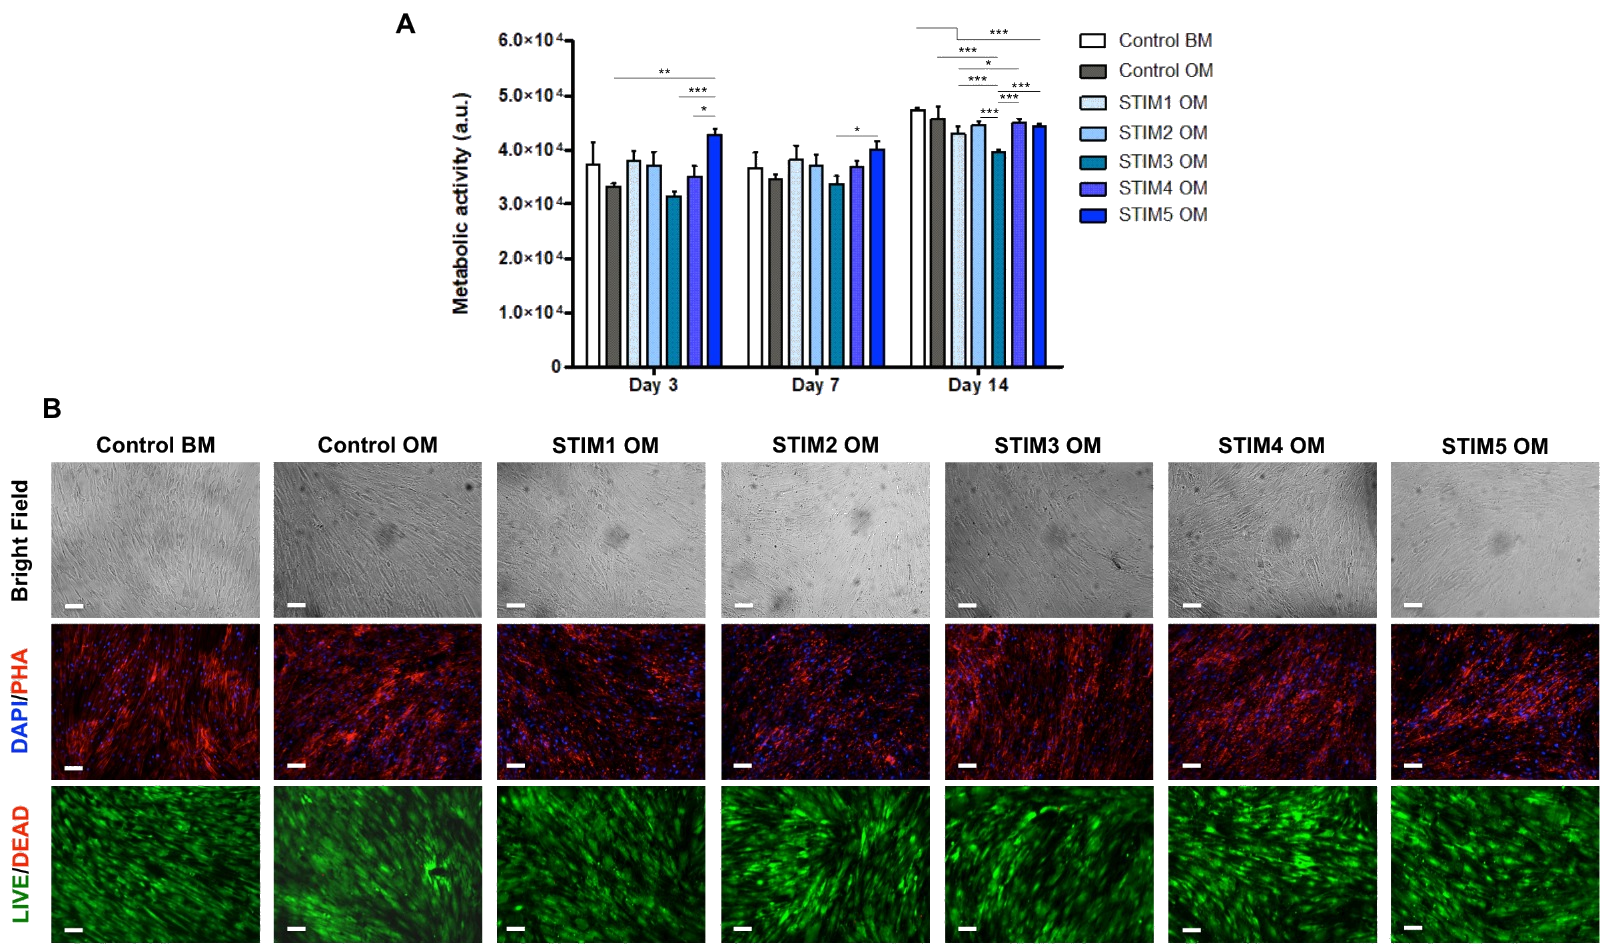
\includegraphics[scale=1.2]{./figures/Figure_4d7.png}}
\caption{Effects of the different electric stimulation protocols on human bone marrow-derived \ac{MSCs} metabolic activity, viability, and morphology. (A) Metabolic activities (determined using the AlamarBlue assay at days 3, 7, and 14) of human bone marrow-derived \ac{MSCs} undergoing osteogenic differentiation under the different electric stimulation protocols. Results are presented as average $\pm$ SD of three ($n=3$) independent experiments. $*p < 0.05; **p < 0.01; ***p < 0.001$. (B) Assessment of cell morphology and viability by Bright Field imaging (top), DAPI/Phalloidin (middle), and LIVE/DEAD (bottom) fluorescent stainings at the end of the experiment (day 14). DAPI stains the nuclei blue, and Phallodin stains the actin cytoskeleton red. In the LIVE/DEAD staining, viable cells are stained in green, while dead cells appear in red. Scale bar: 100 \si{\micro\meter}.}
\label{fig4d7}
\end{sidewaysfigure}
 

\subsection{\acs{ALP} activity, calcium production, and osteogenic stainings} 
To assess the effects of the different electric stimulation protocols on the osteogenic differentiation of human bone marrow-derived \ac{MSCs}, \acs{ALP} activity (Figure \ref{fig4d8}A) and calcium content (Figure \ref{fig4d8}B) quantitative assays were performed on the cultures obtained at the end of the experiment (day 14). As expected, all the conditions (electrically stimulated and non-stimulated) cultured under osteogenic medium presented statistically significant higher \ac{ALP} activities in comparison to the non-stimulated cells cultured under standard growth media conditions (CONTROL BM). Lower \ac{ALP} activity values were observed for the current-based protocol (STIM 3 OM). Nevertheless, this difference was not statistically significant (Figure \ref{fig4d8}A). 

Regarding mineralization, the experimental groups cultured under osteogenic induction conditions present significantly higher calcium contents than the CONTROL BM group (Figure \ref{fig4d8}B). Notably, the current-based electric stimulation protocol (STIM 3 OM) was the only condition that achieved statistically significant higher calcium content (mineralization) than the non-stimulated cells cultured under osteogenic medium (CONTROL OM).

\begin{figure}
\makebox[\textwidth][c]{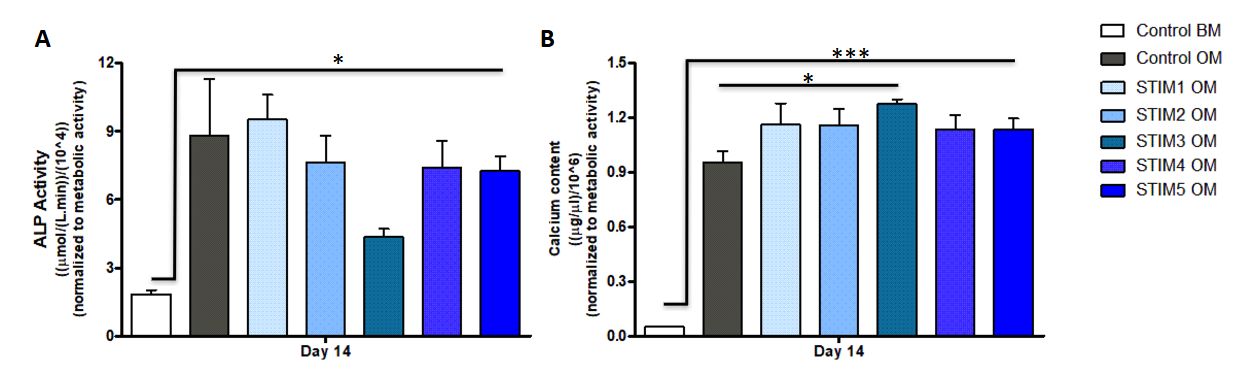
\includegraphics[scale=0.50]{./figures/Figure_4d8.png}}
\caption{(A) \ac{ALP} activity and (B) calcium deposition quantification of human bone marrow-derived \ac{MSCs} cultured under five different electric stimulation protocols after 14 days of osteogenic differentiation. Results are presented as average $\pm$ SD of three ($n=3$) independent experiments. $*p < 0.05; ***p < 0.001$.}
\label{fig4d8}
\end{figure}

The differentiation of human bone marrow-derived \ac{MSCs} towards osteoblasts was further confirmed by the common ALP/Von Kossa, Alizarin Red, and Xylenol Orange osteogenic stainings (Figure \ref{fig4d9}). As expected, all the experimental groups cultured under osteogenic induction medium stained positively for \ac{ALP} activity (top row) and cell mineralization (three bottom rows), demonstrated by the presence of black, red, and fluorescent red mineralized deposits identified by Von Kossa, Alizarin Red and Xylenol Orange stainings, respectively. None or minimal positive osteogenic stainings were observed for the CONTROL BM group. Importantly, all the electric stimulation protocols showed a more intense and spread staining concerning the Alizarin Red staining than the osteogenic non-stimulated group (CONTROL OM). This was particularly evident for the STIM1 OM and STIM3 OM experimental groups. Moreover, Xylenol Orange staining images also suggest a more intense staining for the current-controlled protocol (STIM3 OM).

\begin{sidewaysfigure}
\makebox[\textwidth][c]{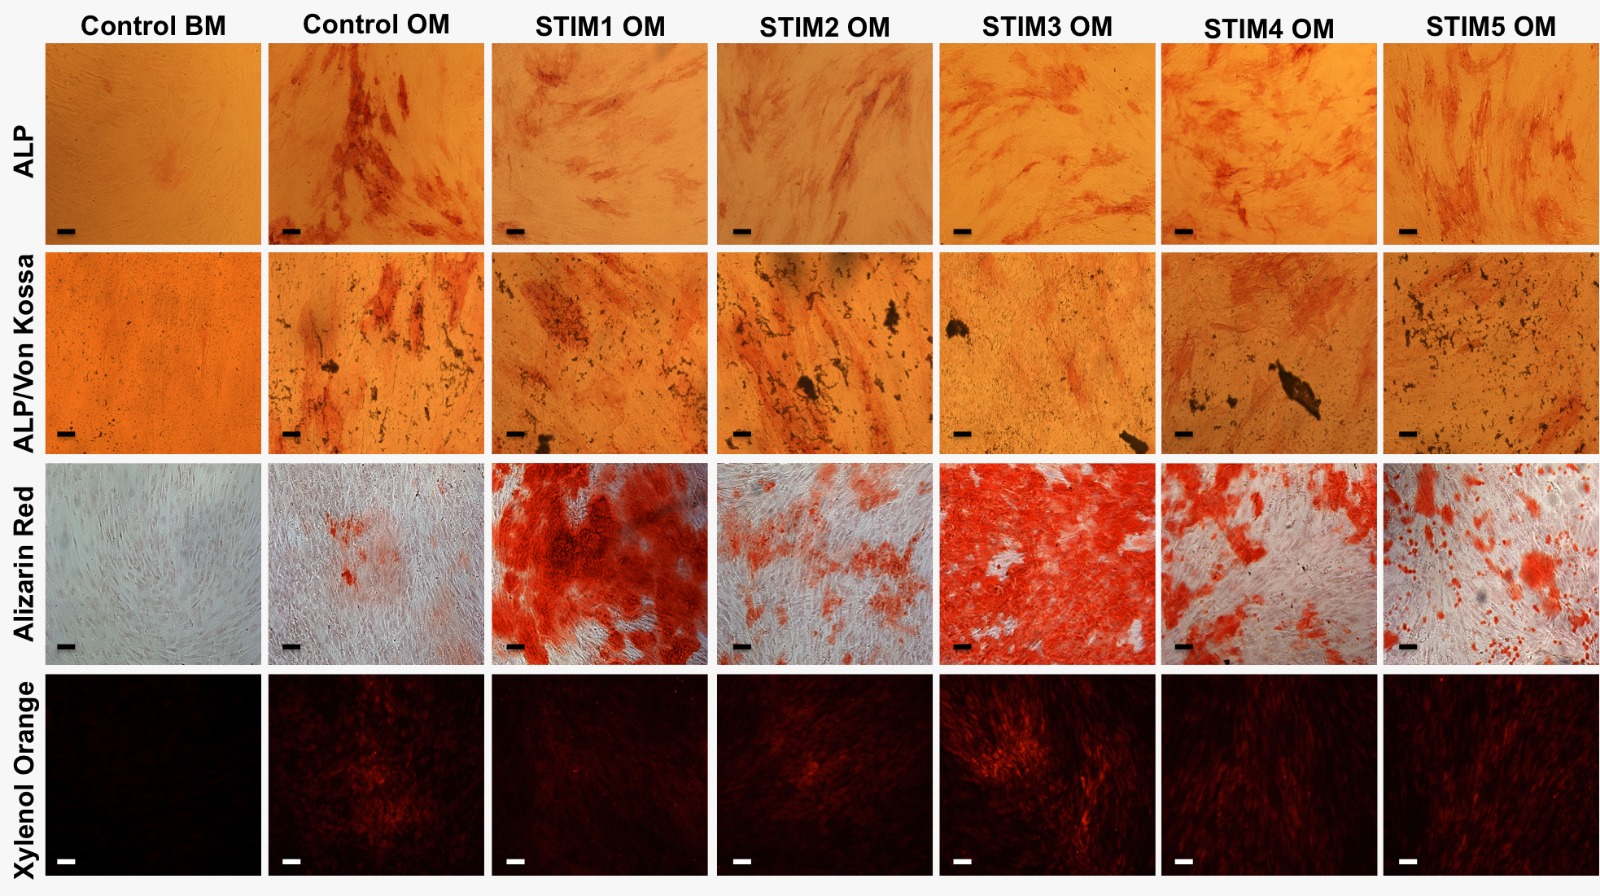
\includegraphics[scale=0.35]{./figures/Figure_4d9.jpeg}}
\caption{ALP, ALP/Von Kossa, Alizarin Red, and Xylenol Orange stainings (from top to bottom rows) of human bone marrow-derived \ac{MSCs} cultured under osteogenic differentiation conditions and exposed to the different electric stimulation protocols for 14 days (and respective non-stimulated controls). \acs{ALP}/Von Kossa staining evidenced the \ac{ALP} activity of the differentiating human bone marrow-derived \ac{MSCs} (reddish areas) and the presence of mineralization (Von Kossa – dark deposits). Alizarin Red staining further confirmed the presence of calcium deposits (red staining). Xylenol Orange fluorescent staining showed the presence of calcium deposits in red. Scale bar: 100 \si{\micro\meter}.}
\label{fig4d9}
\end{sidewaysfigure}   


\subsection{Osteogenic gene expression and immunofluorescence analysis of bone-specific proteins} 
\ac{RT-qPCR} analysis was performed to evaluate the effects of the five different electric stimulation protocols on the expression of bone-specific genes by human bone marrow-derived \ac{MSCs} cultured under osteogenic induction medium for 14 days. As it is possible to observe in Figure \ref{fig4d10}, marker gene expressions were distinctively influenced by the different electric stimulation protocols. ALP (Figure \ref{fig4d10}A) expression was the highest for the non-stimulated CONTROL OM condition, but this difference was only statistically significant concerning STIM2 OM and STIM3 OM groups. All the experimental groups cultured in an osteogenic medium presented significantly upregulated ALP expression in comparison to CONTROL BM. COL1A1 (Figure \ref{fig4d10}B) expression was significantly lower in the STIM3 OM condition than in the other experimental groups. Moreover, the other protocols did not observe statistically significant differences in COL1A1 expression. As expected, the expression of Runx2 (Figure \ref{fig4d10}C) was significantly higher in all the groups cultured under osteogenic induction in comparison to the basal medium condition (CONTROL BM). However, the CONTROL OM group achieved a significantly higher Runx2 expression than all the electric stimulation protocols. OPN (Figure \ref{fig4d10}D) expression was upregulated in all samples cultured in an osteogenic medium in relation to the control BM group. Notably, this late-stage differentiation marker (OPN) expression was significantly higher in STIM3 OM (current) and STIM5 OM protocols when compared to all the other experimental groups cultured under osteogenic induction conditions. OC (Figure \ref{fig4d10}E) expression was the highest in cells cultured under the STIM1 OM protocol. Such upregulated expression was statistically significant compared to all experimental groups except for the STIM3 OM protocol. The gene expressions of CACNA1C and SCN1$\alpha$ - which encode for the 1C subunits of type L of voltage-gated calcium channels and 1$\alpha$ subunit of voltage-gated sodium channels, respectively - were also analyzed due to their known role on the delivery of electrical cues to cells \cite{Li2022-js}. CACNA1C (Figure \ref{fig4d10}F) expression was significantly upregulated in all stimulation protocols in comparison to the non-stimulated conditions (CONTROL BM and CONTROL OM). Moreover, the STIM5 OM condition presented a significantly higher CACNA1C expression than all the other experimental groups. Intriguingly, SCN1$\alpha$ (Figure \ref{fig4d10}G) expression was only significantly upregulated (comparatively to the non-stimulated groups) in the protocols STIM3 OM, STIM4 OM, and STIM5 OM. 

\begin{figure}
\makebox[\textwidth][c]{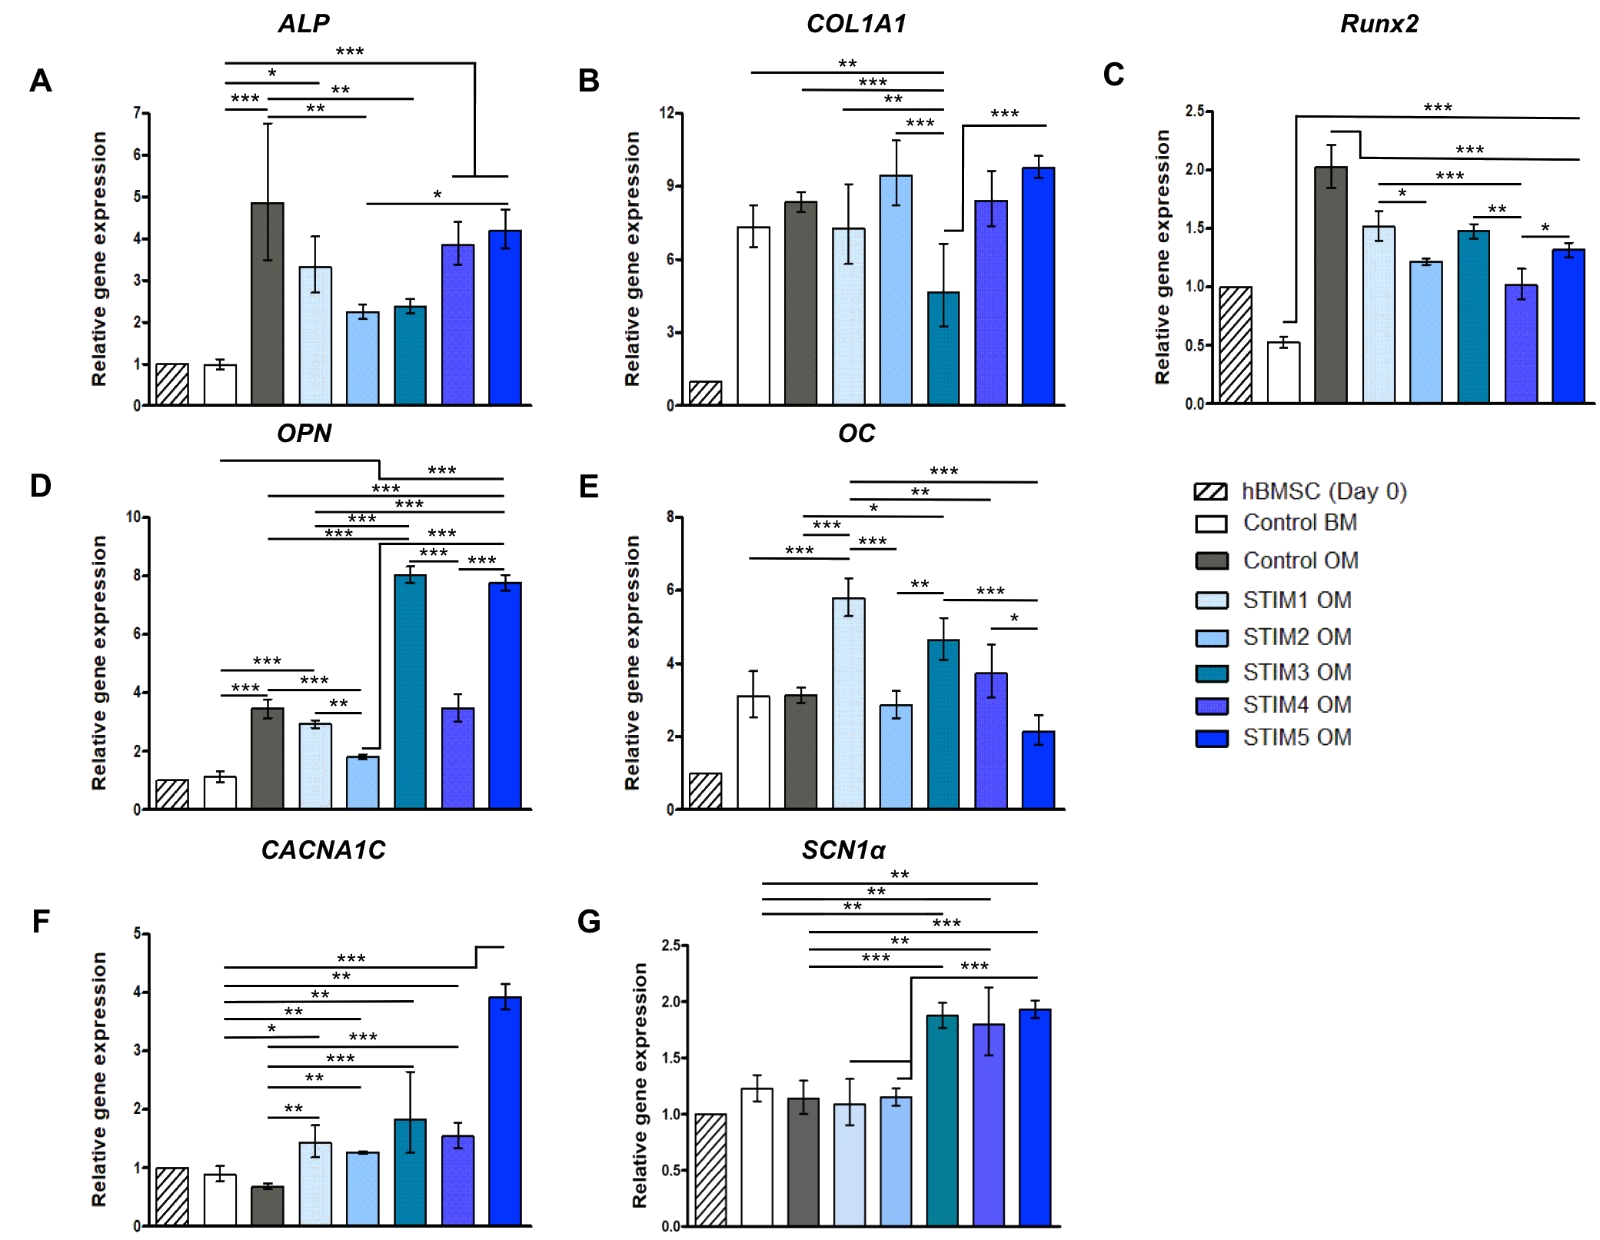
\includegraphics[scale=1.0]{./figures/Figure_4d10.png}}
\caption{Gene expression analysis by RT-qPCR of human bone marrow-derived \ac{MSCs} undergoing osteogenic differentiation under the different electric stimulation protocols for 14 days. Expressions of (A) ALP, (B) COL1A1, (C) Runx2, (D) OPN, (E) OC, (F) CACNA1C, and (G) SCN1$\alpha$ were normalized to the endogenous control GAPDH and calculated as a fold-change relative to the baseline expression of the control sample (hBM-MSCs at day 0). Results are expressed as average $\pm$ SD of three ($n=3$) independent samples. $*p < 0.05; **p < 0.01; ***p < 0.001$.}
\label{fig4d10}
\end{figure}

Immunofluorescence staining of the samples obtained after the osteogenic differentiation of human bone marrow-derived \ac{MSCs} exposed to the five different electric stimulation protocols was performed to assess the presence of the relevant bone \ac{ECM} proteins type I collagen, osteopontin, and osteocalcin. As shown in Figure \ref{fig4d11}, all three proteins (Col I, OPN, OC) were positively identified in all the experimental groups cultured under osteogenic induction conductions, with no noticeable differences in marker intensity expression being observed between the different electric stimulation protocols.

\begin{sidewaysfigure}
\makebox[\textwidth][c]{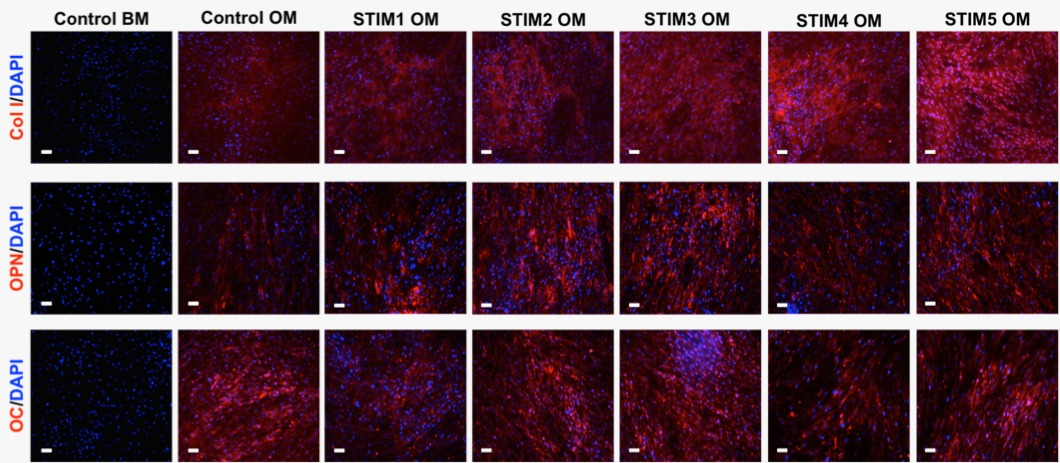
\includegraphics[scale=0.50]{./figures/Figure_4d11.jpg}}
\caption{Immunofluorescence analysis to evaluate the presence of type I collagen (Col I, top), osteopontin (OPN, middle), and osteocalcin (OC, bottom) bone-specific proteins on differentiating human bone marrow-derived \ac{MSCs} cultured under osteogenic induction conditions and exposed to the different electric stimulation protocols for 14 days (and respective non-stimulated controls). Antibody fluorescent staining in the samples appears in red. The samples were counterstained with DAPI, which stains cell nuclei in blue. Scale bar: 100 \si{\micro\meter}.}
\label{fig4d11}
\end{sidewaysfigure}


\section{Discussion}

\subsection{DCoupled setup response characterization and modelling}
An essential difference between direct-coupled systems using electrode/electrolyte interfaces (the system used in this work) and those that use agar salt bridges \cite{Song2007-qr} is that in the latter, only potassium and chloride ions flow from the agar salt bridge into the cell culture region. By contrast, when using immersed electrodes, uncontrolled and unknown free-flowing ions balance the charges by becoming oxidized and reduced in the process, which can unleash unexpected biological effects \cite{Srirussamee2019-ai, Srirussamee2021-cj}. The electrode may also release ions from its material, generating free radicals or being biologically active without further reactions. Stainless steel electrodes can not be considered inert, since they have been previously reported to release ferrous ions when subjected to pulsed stimulation. The ferrous ions release was strongly correlated with waveform parameters and the medium's ionic strength \cite{Tomov2000-db}. Despite this fact, this effect was neglected in the current study because the application of small constant electric currents or low-frequency potential waveforms is expected to release small ionic content into the media. This study unveils the predominant faradaic nature of the electrode/electrolyte interface between the stainless steel 316LVM and the BM or OM, which was established by applying a simple characterization process described by Biesheuvel \textit{et al.} \cite{Biesheuvel2018-wu}. Since our observations result from applying electric potentials inferior to the water hydrolysis limit, we can infer that other cell culture medium chemical species are being oxidized/reduced. This reinforces the importance of further understanding the faradic by-products that are being produced in \ac{DCoupled} stimulations when the electrode material is in direct contact with the culture medium, a necessity also highlighted by \cite{Srirussamee2019-ai, Tomov2000-db}. The average \acs{EF}s generated by our \ac{DCoupled} setup are predicted to be between 1.48 and 0.26 \si{\volt\per\meter}, corresponding to the time-dependent system responses to the input potential step signal, generating a peak electric current (0.17 \si{\milli\ampere}) that immediately drops to a much lower current (0.02-0.03 \si{\milli\ampere}). This peak effect is only observable when applying an electric potential step, since when applying an electric current step, the current source will adjust the electric potential of the electrode terminals in a time-dependent manner. Once the culture medium becomes more/less resistive, the current source will increase/decrease the electric potential at the electrode terminals to maintain the established current. The original \ac{DCoupled} setup from Mobini \textit{et al.} \cite{Mobini2016-jh} was subjected to a current measurement validation in a later work by Srirussamee \textit{et al.} \cite{Srirussamee2019-ai}. When they applied Mobini’s potential of 2.2 \si{\volt} DC, a total current of 0.07 $\pm$ 0.01 \si{\milli\ampere} (mean $\pm$ SD) was measured in each well after it reached a steady state. This measurement corresponds to the dwell phase of the system signal response, as we have observed here. Despite being of identical magnitude to our measured current at the same signal phase (0.02-0.03 \si{\milli\ampere}), the observed difference may arise from the differences in the electrical conductivity of the used culture medium and on the electrode material, which in turn generates a different electrode/electrolyte I-V curve interface relation, as shown in Figure \ref{fig4d5}.   

Since our developed DCoupled setup tries to emulate Mobini's \ac{DCoupled} setup, we also numerically modeled Mobini \textit{et al.} setup \cite{Mobini2016-jh} using the same methodology, considering their reported geometry and the posterior measured electric current by Srirussamee \textit{et al.}. We also took advantage of known typical electrical material properties for titanium, polystyrene, and culture medium. The average predicted \acs{EF} in Mobini's setup is 0.59 \si{\volt\per\meter} for the culture medium volume. This predicted electric field is lower than the reported by Mobini \textit{et al.} \cite{Mobini2016-jh} original setup and by other subsequent studies using the same setup \cite{Mobini2017-wp, Mobini2017-zr, Leppik2018-bw}, which report that a potential step of 2.2 \si{\volt} DC generated 100 \si{\volt\per\meter}. This value is contradicted by Srirussamee \textit{et al.} current measures (2019) \cite{Srirussamee2019-ai}, later repeated with more detail \cite{Srirussamee2021-cj} and with an additional potential measure at two distant points (8 \si{\milli\meter} apart) in the culture medium.

From Figure 2 in Srirussamee \textit{et al.} \cite{Srirussamee2021-cj} and with the help of a digitizer, the voltage drop between those two points can be estimated to be 0.0169 \si{\volt} (A: 0.8125 \si{\volt}, B: 0.7956 \si{\volt}). This potential measurement allows us to grossly estimate the \acs{EF} to be 2.1 \si{\volt\per\meter}, a magnitude value closer to our estimate. The difference between this value and the ones presented in our study may rely on the unknowns of the exact properties of the culture medium and the exact geometry of the electrodes and liquid volume used. Nevertheless, the measurements from Srirussamee \textit{et al.} \cite{Srirussamee2019-ai} and Tomov \textit{et al.} \cite{Tomov2000-db} reinforce the confidence in our delivered \ac{EF} prediction methodology. Also, the study from Zimmermann \textit{et al.} \cite{Zimmermann2021-fx}, describing the application of digital models to monitor and control electrical stimulation \textit{in vitro}, considered a stimulation chamber similar to the Mobini \textit{et al.} setup \cite{Mobini2016-jh}. Results from their \ac{DCoupled} model for Mobini’s DC stimulation conditions predicted an \ac{EF} of 0.33 \si{\volt\per\meter}, following Srirussamee \textit{et al.} \cite{Srirussamee2021-cj} current density predictions (0.5 \si{\ampere\per\square\meter}). That prediction agrees with our model calculations for Mobini’s \ac{EF} magnitude (0.59 \si{\volt\per\meter}), differing from the values of 100 \si{\volt\per\meter} reported by Mobini \textit{et al.}. Regarding \ac{DCoupled} stimulation regimes using directly immersed electrodes, agar-salt bridges, or a conductive scaffold substrate, a mandatory reading for further understanding of the electrochemistry effects in each setup is the theoretical analysis of Guette-Marquet \textit{et al.} \cite{Guette-Marquet2021-rp}. Their analysis also suggests that, for two-electrode systems (like the one used here), many reported \ac{EF} magnitude values have been overestimated, which is also in line with Zimmermann \textit{et al.} \cite{Zimmermann2021-fx} and our predictions. Guette-Marquet \textit{et al.} also advises changing experimental practices by applying current instead of voltage, a condition that we implemented in the protocol condition STIM3 OM. We monitored and reported the resultant electric current for the remaining potential conditions. Although we have used a direct probing method (multimeter) to measure the electric current that passes through the system, indirect probing methods should be privileged in the future to avoid direct influence in effects, like the Rogowski-coil method of measuring electric current \cite{Ward1993-wl}.


\subsection{Effects of different electric stimulation protocols on \ac{MSCs} osteogenic differentiation}
The successful clinical outcomes of electric stimulation in bone healing strategies encouraged the scientific community to try to understand its underlying mechanisms at the cellular and molecular levels. Electric stimulation has been previously applied to enhance the osteogenic differentiation of \ac{MSCs} \textit{in vitro} \cite{Guillot-Ferriols2022-wn, Peng2023-ud, Bianconi2023-rs}. However, the cellular processes/signaling pathways by which electric stimulation regulates osteogenesis are still poorly understood. Therefore, there is no optimal, defined, standardized electric stimulation protocol for inducing \ac{MSCs} osteogenic commitment \textit{in vitro}. Many studies using poorly characterized experimental systems for electric stimulation limit the comparison of results and protocol reproducibility. Existing studies often use single voltage-controlled protocols to treat \ac{MSCs} without using numerical modelling to visualize the output of the selected stimulation parameters. They usually analyze the results only by comparing them to non-stimulated controls, unable to compare their results with other existent works. Moreover, current-based electric stimulation protocols imposing current intensity instead of voltage is vastly unexplored \cite{Guette-Marquet2021-rp}.

Thus, in this study, we aimed to directly compare different potential-controlled electric stimulation protocols with a current-controlled one in terms of their capacity to improve the in vitro osteogenesis of human bone marrow-derived \ac{MSCs}. The \ac{EF} magnitude calculation performed will allow us to compare this work output with similar future studies. All the electric stimulation protocols resulted in final cell cultures with high viability, high metabolic activity, and regular cell morphology (Figure \ref{fig4d7}). These results follow the study from Zhao \textit{et al.} \cite{Zhao2011-wy}, which reported high cell viabilities (90-95\%) and typical elongated fibroblast-like morphology for human bone marrow-derived \ac{MSCs} exposed to \ac{EFs} of 200 \si{\milli\volt\per\milli\meter} (two orders of magnitude higher than the \ac{EFs} applied in this work). Regarding the applied current-controlled protocol (STIM3 OM), the overtime increase in metabolic activity (indirect measure of cell proliferation, AlamarBlue assay) observed in Figure \ref{fig4d7}A and high cell viability/regular cell morphology (Figure \ref{fig4d7}B) are concordant with the results reported by Shao \textit{et al.} \cite{Shao2011-dz} for osteoblasts exposed to DCoupled electric stimulation of 100 \si{\micro\ampere} (4 \si{\hour} per day) for six days.

The effects of the different electric stimulation protocols on the human bone marrow-derived \ac{MSCs} osteogenic differentiation were assessed after 14 days through the quantification of ALP activity and calcium production (Figure \ref{fig4d8}), typical osteogenic stainings (Figure \ref{fig4d9}), bone-related marker genes expression (Figure \ref{fig4d10}) and immunofluorescence analysis of essential bone ECM proteins (Figure \ref{fig4d11}). Our results suggested an advantageous performance of the applied current protocol (STIM3 OM) in enhancing calcium production/mineralization by osteogenic differentiating human bone marrow-derived \ac{MSCs} (Figure \ref{fig4d8}B). This result concurs with the more intense and spread Alizarin Red and Xylenol Orange stainings observed in Figure \ref{fig4d9} for the cultures exposed to STIM3 OM protocol. Moreover, the higher mineralization observed for the applied current electric stimulation condition is supported by the previous study performed by Zhang \textit{et al.} \cite{Zhang2016-ul}, in which significantly higher calcium deposition was obtained (at day 14) for human adipose-derived \ac{MSCs} cultured on polypyrrole/polycaprolactone scaffolds under osteogenic induction and exposed to 200 \si{\micro\ampere} of direct current for 4 \si{\hour} per day.

All the electric stimulation protocols resulted in similar or lower ALP activities (Figure \ref{fig4d8}A) and \textit{ALP} (Figure \ref{fig4d10}A), \textit{Runx2} (Figure \ref{fig4d10}C) gene expressions than the non-stimulated Control OM group. Such observation might be explained by the fact that \textit{Runx2} and \textit{ALP} expressions (and respective ALP activity) are more predominant in the initial phase of MSC’s osteogenic differentiation (early markers) that precede the mineralization phase, after which their levels decrease \cite{Beck2003-fx}. Thus, it is possible that electric stimulation protocols promoted a faster osteogenic differentiation (as supported by the enhanced mineralization (Alizarin Red staining, Figure \ref{fig4d9}), upregulation of late-stage markers (\textit{OPN} (Figure \ref{fig4d10}D) and \textit{OC} (Figure \ref{fig4d10}E)) expression and respective proteins presence in Figure \ref{fig4d11}), resulting in the observed lower \textit{Runx2} and \textit{ALP} expressions.

OPN has been shown to play a pivotal role in regulating calcium phosphate nucleation during the mineralization process \cite{Liu2020-zx}. Thus, the significantly higher \textit{OPN} gene expression observed in Figure \ref{fig4d10}D for the cultures exposed to STIM3 OM protocol is well correlated with the enhanced mineralization obtained for the same condition (Figure \ref{fig4d8}B and Figure \ref{fig4d9} - Alizarin Red and Xylenol Orange stainings). This beneficial effect of applied current electric stimulation on \textit{OPN} expression and mineralization has been previously reported \cite{Zhang2016-ul}. \textit{OC} gene upregulated expression has also been associated with improved bone mineralization \cite{Zoch2016-bn}. Therefore, the significantly higher \textit{OC} expressions obtained for the experimental groups STIM1 OM and STIM3 OM might explain these conditions’ improved calcium production (Figure \ref{fig4d8}B) and more intense mineral deposition (Alizarin Red staining, Figure \ref{fig4d9}).

\textit{CACNA1C} gene role in the signaling cascade regulating the osteogenic differentiation of human MSCs and subsequent tissue mineralization has been demonstrated in previous works \cite{Zhang2016-ul}. Zhang \textit{et al.} showed the superior role of voltage-gated calcium channels in the modulation of adipose-derived \ac{MSCs} in comparison to other ionic channels (sodium, potassium, and chloride) \cite{Zhang2016-ul}. Moreover, the study from Camarero-Espinoza and Moroni further evidenced the correlation between \textit{CACNA1C} and the osteogenic differentiation of human bone marrow-derived \ac{MSCs}, as they showed that blocking the activity of \textit{CACNA1C} resulted in a downregulation of the bone-specific genes (\textit{Runx2}, \textit{COL1A1} and \textit{OC}) \cite{Camarero-Espinosa2021-dh}. Previous studies have proposed that electric stimulation promoted the increase of cytosolic calcium ionic concentration both in osteoblasts and \ac{MSCs}, which subsequently activates voltage-gated calcium channels and regulates cell functions via calmodulin pathways \cite{Zhang2016-ul, Zayzafoon2006-vc}. Accordingly, our results showed that all the electric stimulation protocols resulted in the upregulation of \textit{CACNA1C} expression (Figure \ref{fig4d10}F) with the highest levels observed for the STIM5 OM condition. STIM5 OM protocol also promoted the highest \textit{COL1A1} expression (Figure \ref{fig4d10}B), which is in line with the relation between \textit{CACNA1C} and \textit{COL1A1} genes previously suggested in the study from Camarero-Espinoza and Moroni \cite{Camarero-Espinosa2021-dh}.

The different electric stimulation protocols employed resulted in distinct cellular responses, particularly regarding \ac{MSCs} gene expression profiles (Figure \ref{fig4d10}). Considering the protocols STIM1 OM (1 hour, Higher \ac{EF}+Lower \ac{EF}) and STIM2 OM (1 second, Higher \ac{EF}), it appears that a single pulse of high \ac{EF} (STIM2 OM) is sufficient to achieve \textit{ALP}, \textit{COL1A1}, \textit{CACNA1C} and \textit{SCN1$\alpha$} expressions similar to STIM1 OM. However, a more prolonged stimulation (prevalence of the Lower \ac{EF} signal component) seems to be advantageous for higher expressions of more mature marker genes (\textit{OPN} and \textit{OC}) and mineralization (intense and spread Alizarin Red staining, Figure \ref{fig4d9}), suggesting a more advanced differentiation stage achieved by the cells exposed to STIM1 OM than STIM2 OM. This effect is also observed comparing a single pulse of high \ac{EF} (STIM2 OM) with multiple pulse protocols (STIM4 OM and STIM5 OM), in which the latter resulted in higher levels of bone-specific gene expression. Statistical significant differences in gene expression levels (\textit{Runx2}, \textit{OPN}, \textit{OC} and \textit{CANA1C}) were also observed between the protocols STIM4 OM (1 hour, sequence of multiple Higher \ac{EF} + short duration Lower \ac{EF}) and STIM5 OM (1h, sequence of multiple Higher \ac{EF} + short duration Lower \ac{EF}, with five times more pulses than STIM4 OM), suggesting the relevance of the signal period/frequency in the modulation of \ac{MSCs} osteogenic differentiation. Concordantly, Wang \textit{et al.} \cite{Wang2016-ff} study showed that different frequencies of electric stimulation lead to distinct outcomes in the \textit{in vitro} osteogenesis of MC3T3-E1 pre-osteoblastic cells.

In general, our results (higher mineralization and \textit{OPN} gene expression) suggest the benefits of using a current-controlled electric stimulation protocol (STIM OM3) for the in vitro stimulation of \ac{MSCs} towards the bone lineage. We are aware that this improved performance in STIM3 OM may result from the potential signal oscillation at the electrodes that, when trying to support the prescribed current, increased the potential above 1.2 \si{\volt}, which probably generated uncontrolled and unknown redox artifacts that might influence \ac{MSCs} response. Previous studies have reported the role of reactive oxygen products on the enhancement of MSC osteogenic differentiation \cite{Srirussamee2021-cj, Sheppard2022-gj}. Despite this limitation, our work provides valuable insights towards the \textit{in silico} and \textit{in vitro} optimization of electric stimulation protocols for producing high-quality clinically relevant \ac{MSCs}-based \ac{BTE} products for bone repair treatments.

Future work will include further optimization of the applied current-controlled electric stimulation protocols toward improved osteogenesis combined with whole transcriptome analysis. This will allow the unraveling and understanding of underlying molecular mechanisms/signaling pathways by which current-controlled electric stimulation modulates \ac{MSCs} osteogenesis. Those electric stimulation protocols could also be applied to basal medium cultures to find if an electric stimulus on its own could replace the addition of osteogenic promoters. Developing new scalable devices for electric stimulation to allow a middle/high-throughput analysis will also be considered.


\section{Summary}

This chapter points out that the custom-developed \acs{DCoupled} system will generate redox reactions in the electrode/electrolyte interface even for potential differences inferior to the water electrolysis limit, observable by the characteristic system's electric wave response. So, once unknown chemical species present in the medium solution are oxidized or reduced, \acs{DCoupled} systems like this one may generate uncontrollable and unpredictable cellular interactions, which, in turn, will hamper the conclusions regarding the effects of the applied \acs{EF}. 

A numerical \acs{FEM} digital model of the cell culture condition and \acs{DCoupled} system was employed to characterize and predict the magnitude distribution of the electric fields generated by the different stimulation protocols. The models successfully assessed the impact of small culture medium volume and electrode geometrical variations on the delivered \acs{EF}. Performed \textit{in vitro} cell culture studies showed that all the electric stimulation protocols applied did not cause any impairment in cell viability and morphology, effectively supporting the osteogenic differentiation of human bone marrow-derived \ac{MSCs}. Differences observed in the provoked cellular effects between all the applied protocols conclude that osteogenic gene expression was promoted in all protocols when compared to osteogenic media control regarding the expression of COL1A1, CACNA1C, SCN1$\alpha$. Applying just a single higher \acs{EF} signal phase does not affect ALP activity and calcium content. However, increasing the number of times this signal was applied increased the gene expression of APL, Osteopontin, CACNA1C, and SCN1$\alpha$ correspondingly. Moreover, it is important to notice that applying different stimulation protocol parameters has been shown to promote different gene expression conditions.  

Despite the practical nature of \acs{DCoupled} setups and their capabilities as a tool to promote osteogenesis, this thesis moved on to a more reliable capacitive coupled stimulation system that guarantees stimulation without electron transfer processes. Thus bypassing the unresolved faradaic uncertainties associated with \acs{DCoupled} systems that were observed in this chapter.


%\newpage
%\bibliography{library_c4b} 
%\bibliographystyle{plain}
%\end{document}